% \documentclass[review,12pt]{elsarticle}
\documentclass[5p,times]{elsarticle}
%% Journal name
\journal{Computerized Medical Imaging and Graphics}

%% -- Packages ----------------------------------------------------------------
\usepackage[utf8]{inputenc}
\usepackage{graphicx}
\usepackage{amsmath,amssymb}
\usepackage{booktabs}
\usepackage{multirow}
\usepackage{url}
\usepackage{xcolor}
\usepackage{enumitem}
\usepackage{float}
\usepackage{microtype}

%% hyperref --- load after elsarticle internals
\usepackage{hyperref}
\hypersetup{
  colorlinks = true,
  linkcolor  = blue!70!black,
  citecolor  = blue!70!black,
  urlcolor   = blue!70!black
}

%% -- Custom commands ----------------------------------------------------------
\newcommand{\ie}{\textit{i.e.}}
\newcommand{\eg}{\textit{e.g.}}
\newcommand{\etal}{\textit{et al.}}
\newcommand{\malariai}{\textsc{MalariAI}}

\begin{document}

\begin{frontmatter}

\title{\texorpdfstring{\malariai}{MalariAI}: A Label-Resilient Decoupled Framework for Universal
  Cell Segmentation and Explainable Stage Classification in Dense Malaria
  Blood Smears}

%% Authors and affiliations
\author[1]{Kaysarul Anas Apurba\corref{cor1}}
\ead{Kaysarulanas2@gmail.com}
\cortext[cor1]{Corresponding author.}

\author[1]{Md Hasibul Hasan}

\author[2]{Mohammad Ali}

%% Primary Affiliations (Current Status for APC Waiver evaluation)
\address[1]{Independent Researcher, Dhaka, Bangladesh}
\address[1]{Independent Researcher, Dhaka, Bangladesh}

%% Permanent/Past Academic Addresses (Historical context)
\fntext[fn1]{Authors Apurba and Hasan were previously with the Faculty of Science, Engineering and Architecture, Laurentian University, Sudbury, Ontario, Canada.}
\fntext[fn2]{Author Ali was previously with the Melbourne Institute of Technology, Melbourne, Australia.}

%% -- Abstract ----------------------------------------------------------------
\begin{abstract}
Automated malaria diagnosis from peripheral blood smear microscopy remains
a critical unsolved problem in global health AI, particularly in
resource-limited settings where expert microscopists are scarce. Despite
significant progress in applying deep learning to this domain, three
compounding failure modes persist across the published literature. First,
end-to-end object detectors treat unannotated cells as background during
training, producing recall figures that are an artefact of annotation
completeness rather than true cell recovery. Second, Non-Maximum Suppression
(NMS) systematically discards valid detections in the dense smear regions
where infection counts matter most. Third, all existing whole-slide
detection pipelines produce opaque class labels with no spatial evidence,
severely limiting clinical trust and adoption. We present \malariai{}, a
two-stage decoupled framework that addresses all three failure modes in
a unified, deployable pipeline. Stage~1 applies an annotation-agnostic
distance-transform guided watershed algorithm to isolate every cell in a
full 1600$\times$1200 blood smear image, recovering 75.95\% of annotated
cells across the 120-image NIH BBBC041 test set without consulting any
ground-truth label. Stage~2 applies a fine-tuned EfficientNet-B0
classifier trained with Focal Loss ($\gamma = 2.0$, per-class inverse
frequency weights) on 64$\times$64 crops, achieving 98.36\% overall
classification accuracy on the validation split with per-class accuracy
of 87.5\% (schizont) and 75.0\% (gametocyte) --- rare stages for which
a Faster R-CNN baseline achieves only 24.57\% and 25.95\% AP respectively.
Grad-CAM\texttt{++} spatial heatmaps are generated for every detected cell
as an integrated clinical explainability layer. We benchmark \malariai{}
against a Faster R-CNN (ResNet-50 FPN) baseline trained for 80 epochs on
NIH BBBC041 (mAP@0.5 = 58.99\%), demonstrating that architectural
decoupling between segmentation and classification is a principled,
measurable response to the incomplete-annotation problem inherent in
real-world malaria datasets, and that integrated spatial explainability is
achievable without sacrificing classification performance.
\end{abstract}

%% -- Keywords ----------------------------------------------------------------
\begin{keyword}
Malaria detection \sep
Blood smear analysis \sep
Instance segmentation \sep
Watershed algorithm \sep
EfficientNet \sep
Focal Loss \sep
Explainable AI \sep
Grad-CAM\texttt{++} \sep
Medical image analysis \sep
Decoupled framework
\end{keyword}

\end{frontmatter}

%% ============================================================================
%% SECTION 1 -- INTRODUCTION
%% ============================================================================
\section{Introduction}
\label{sec:intro}

Malaria remains one of the most consequential infectious diseases in
contemporary global health. The World Health Organization reported 249
million cases worldwide in 2022, resulting in an estimated 608,000 deaths,
of which 95\% occurred in sub-Saharan Africa~\cite{who2023}. The burden
falls disproportionately on children under five years of age and on
populations with limited access to diagnostic infrastructure. Despite the
existence of effective antimalarial therapies, a fundamental bottleneck
persists at the point of diagnosis.

The clinical gold standard for malaria diagnosis is microscopic examination
of a Giemsa-stained peripheral blood smear under a 100$\times$ oil-immersion
objective. A trained microscopist inspects the slide, identifies red blood
cells (RBCs) infected by \textit{Plasmodium} parasites, and estimates the
parasite stage from cellular morphology. The parasite lifecycle stage ---
ring, trophozoite, schizont, or gametocyte --- carries direct implications
for treatment selection and disease severity assessment~\cite{delves2012}.
This manual process requires 20--30 minutes per slide, specialised training
that takes years to acquire, and physical equipment that is not universally
available in endemic regions. The result is a diagnostic bottleneck that
costs lives.

The promise of deep learning for automated malaria diagnosis has generated
substantial research interest over the past decade~\cite{poostchi2018}.
Convolutional neural networks (CNNs) have demonstrated strong performance
on cell-patch classification tasks~\cite{rajaraman2019, singh2025}, and
end-to-end object detectors such as Faster R-CNN~\cite{ren2015} and
YOLO~\cite{yolov4malaria2024} have been applied to the whole-slide detection
problem. However, no single published system has achieved the combination
of properties required for genuine clinical deployment: annotation resilience,
dense-region recall, multi-class stage classification, and integrated
spatial explainability.

Our analysis of the existing literature identifies three specific, measurable
failure modes that collectively prevent any current system from being
clinically deployable:

\begin{description}[leftmargin=2em]
  \item[\textbf{P1 --- Incomplete Annotation.}] The NIH BBBC041 benchmark
  --- the de~facto standard for malaria detection research --- annotates
  only infected cells and a subset of healthy RBCs. End-to-end detectors
  trained on this data learn to treat unannotated cells as background,
  producing false positives on any cell the annotators happened to skip.
  Validation loss in such systems plateaus early and subsequently
  \emph{increases}, a pattern our Baseline A experiments confirm and
  diagnose as a structural consequence of label incompleteness rather than
  model overfitting.

  \item[\textbf{P2 --- Dense Overlap and NMS Failure.}] Our exploratory
  analysis of BBBC041 finds that 58\% of training images contain at least
  one ground-truth pair with $\text{IoU} > 0.3$, with a maximum of 223
  annotated cells per image. All anchor-based detectors apply Non-Maximum
  Suppression (NMS) to filter proposals, but NMS assumes overlapping
  proposals are duplicates of the same object. In dense smear regions, this
  assumption fails, causing systematic deletion of true positive detections.

  \item[\textbf{P3 --- Black-Box Output.}] Every published whole-slide
  malaria detection system returns a class label. None produce spatial
  evidence of the prediction that clinicians could use to validate,
  audit, or override the system output~\cite{selvaraju2017,chattopadhyay2018}.
  XAI applications in the malaria literature are confined to pre-isolated
  patch classifiers; integration into a detection pipeline operating on
  full blood smear images has not been achieved.
\end{description}

We present \malariai{}, a two-stage decoupled framework that structurally
eliminates all three failure modes. The key insight is that cell
\emph{localisation} and cell \emph{classification} are biologically
distinct sub-problems that benefit from different inductive biases.
By separating them into sequential, independently optimised stages,
\malariai{} avoids the annotation dependency of end-to-end detection
(P1), eliminates the NMS step entirely (P2), and enables per-cell
spatial explainability to be applied after classification (P3).

\medskip
\noindent\textbf{Contributions.} This paper makes three concrete contributions:

\begin{enumerate}[leftmargin=*, label=\textbf{C\arabic*.}]
  \item \textbf{Label-Resilient Cell Segmentation (C1).}
    An annotation-agnostic Stage~1 based on distance-transform guided
    watershed recovers 75.95\% of ground-truth cells on the 120-image
    BBBC041 test set \emph{without consulting any annotation}, structurally
    eliminating Problem~P1 from the pipeline.

  \item \textbf{Density-Invariant Instance Separation (C2).}
    Distance-transform watershed operates at the morphological level
    and never applies NMS. Touching cells in dense smear regions are
    separated at the instance level by the distance-transform topology,
    structurally eliminating Problem~P2.

  \item \textbf{Integrated End-to-End Spatial Explainability (C3).}
    Grad-CAM\texttt{++} heatmaps are generated for every cell detected
    in a full blood smear image, producing a two-view output: a 160-pixel
    crop overlay and a full-image heatmap localising all parasite
    activations simultaneously. To our knowledge, this is the first
    whole-slide malaria detection system to integrate per-cell spatial
    explainability as a first-class output.
\end{enumerate}

\medskip
\noindent\textbf{Paper organisation.}
Section~\ref{sec:related} reviews the related literature across five thematic
areas. Section~\ref{sec:method} describes the dataset, both pipelines, and
evaluation metrics. Section~\ref{sec:experiments} presents quantitative and
qualitative results. Section~\ref{sec:discussion} discusses implications and
limitations. Section~\ref{sec:conclusion} concludes with directions for future
work. An appendix details the iterative development of the inference pipeline.

%% ============================================================================
%% SECTION 2 -- RELATED WORK
%% ============================================================================
\section{Related Work}
\label{sec:related}

We organise the literature into five thematic areas: (i)~classical and
feature-based approaches, (ii)~CNN-based classification on pre-isolated
cells, (iii)~end-to-end object detection and instance segmentation,
(iv)~two-stage decoupled pipelines, and (v)~explainable AI for clinical
malaria diagnosis. We conclude with a cross-cutting analysis of open
problems.

\subsection{Classical and Feature-Based Approaches}
\label{ssec:classical}

Early automated malaria diagnosis relied on carefully engineered image
processing pipelines applied to Giemsa- or May--Gr\"{u}nwald--Giemsa
(MGG)-stained blood smears. The dominant approach combined global
thresholding (\eg, Otsu's method~\cite{otsu1979}), morphological
operations such as erosion and dilation, and hand-crafted feature
descriptors (\eg, shape moments, colour histograms, Gabor texture
features) fed into classical classifiers such as Support Vector Machines
(SVM) or Random Forests~\cite{poostchi2018}.

These pipelines established a fundamental insight that malaria detection
is a two-phase problem: cells must first be localised before their internal
morphology can be assessed. However, they suffered from two compounding
weaknesses. Segmentation quality degraded sharply when cells overlapped,
and hand-crafted features failed to generalise across staining protocols,
microscope configurations, and acquisition sites~\cite{poostchi2018,delgado2020}.
Nonetheless, classical watershed segmentation based on the distance
transform~\cite{beucher1992} remains competitive for the cell
\emph{localisation} sub-problem: it requires no labelled training data,
its convergence is deterministic, and it is naturally suited to the circular
morphology of red blood cells. This motivates our adoption of
distance-transform watershed as Stage~1.

\subsection{CNN-Based Classification of Pre-Isolated Cells}
\label{ssec:cnn_class}

The release of the NIH malaria cell image dataset~\cite{rajaraman2019},
comprising individually cropped and labelled cell patches, catalysed CNN
classification studies. Rajaraman \etal~\cite{rajaraman2019} evaluated
fine-tuned architectures (VGG-16, ResNet-50, Xception) and found that
transfer learning from natural image corpora substantially outperformed
training from scratch.

More recently, Singh \etal~\cite{singh2025} propose an optimised hybrid
framework combining a 12-layer CNN with EfficientNet-B7 through a parallel
feature-fusion head. Otsu-based preprocessing of the RGB images enhances
parasite-relevant regions before classification, yielding 97.96\% accuracy
on their 43,400-image dataset. Segmentation quality on a manually annotated
100-image subset achieves a Dice coefficient of 0.848 and Jaccard Index
of 0.738. The approach is conceptually related to our Stage~2 design, but
it operates exclusively on pre-cropped, individually isolated cell patches.
The cell isolation problem --- finding cells in a dense, unannotated whole
slide --- is absent. The authors explicitly acknowledge that
``interpretability tools need to be refined to become clinically
applicable'' and identify real-time deployment as future work~\cite{singh2025}.

This family of work collectively avoids the hard sub-problem of whole-slide
cell detection. Reported accuracy metrics measure only classification on
pre-isolated patches and cannot be compared to detection system benchmarks.

\subsection{End-to-End Object Detection and Instance Segmentation}
\label{ssec:e2e}

The Faster R-CNN architecture~\cite{ren2015} --- combining a Region Proposal
Network (RPN) with a two-stage classification head over a ResNet-FPN
backbone --- was among the first deep learning systems applied directly to
the whole-slide malaria detection problem. Hung \etal~\cite{hung2018}
demonstrated high accuracy using a cascaded Faster R-CNN with an AlexNet
backbone, establishing the feasibility of end-to-end detection. Subsequent
work has explored lighter architectures: optimised YOLOv4 models with
backbone replacement and layer pruning achieve strong mAP on thin
smear images~\cite{yolov4malaria2024}.

Instance segmentation --- producing a pixel-level mask per detected cell
--- was explored by Loh \etal~\cite{loh2021} using Mask R-CNN~\cite{he2017maskrcnn}.
Their model achieves inference speeds 15$\times$ faster than manual counting.
These results represent the closest prior art to our Baseline A evaluation.

However, end-to-end detectors exhibit two systematic failure modes in the
malaria domain. First, all such models operate under the closed-world
assumption: any region without a ground-truth bounding box is treated as
background during training. In NIH BBBC041, annotation is incomplete; a
detector trained on this data suppresses unannotated cells, producing recall
figures that reflect annotation density rather than true cell recovery rate.
Loh \etal~\cite{loh2021} acknowledge this, proposing semi-automated
labelling to reduce annotation bias.

Second, Non-Maximum Suppression (NMS) calibrated for non-overlapping objects
fails in dense smear regions where genuine cells share high IoU. Rather than
solving this, prior work filters out dense images before evaluation~\cite{loh2021},
sacrificing exactly the images where automated diagnosis is most needed.

\subsection{Two-Stage Decoupled Pipelines}
\label{ssec:twostage}

The closest architectural precedents to \malariai{} separate cell
segmentation from cell classification into sequential stages.

\textbf{Delgado-Ortet \etal}~\cite{delgado2020} present a three-stage
pipeline comprising a SegNet-based~\cite{badrinarayanan2017} segmentation
network, a crop-and-mask stage, and a 13-layer CNN classifier, achieving
93.72\% global segmentation accuracy and 87.04\% malaria detection
specificity on MGG-stained smears. The work demonstrates decoupled pipeline
viability but suffers from three failures: the segmentation network
misclassifies leukocytes and platelets, inducing cascading classification
errors; the classifier overfits from 95.0\% validation to 75.39\% test
accuracy due to a five-patient training set; and class imbalance is
unaddressed. Their stated future work --- annotating more cell classes,
generating larger datasets, mixing data across institutions~\cite{delgado2020}
--- reads as a near-complete specification of the improvements we implement.

\textbf{Pandiaraj \etal}~\cite{pandiaraj2024} combine a
Trans-MobileUNet\texttt{++} segmentation network with an Adaptive and
Atrous Convolution-based Recurrent MobileNetV2 detection backbone, reporting
94.88\% accuracy on Kaggle-hosted pre-cropped cell image datasets. The
framework performs binary classification only (parasitised vs.\ uninfected),
does not operate on whole blood smear images, and reports no mAP metric at
any IoU threshold, precluding quantitative comparison with detection system
benchmarks. The metaheuristic optimisation introduces reproducibility
concerns: sensitivity to random initialisation and absence of convergence
guarantees make independent replication impractical~\cite{pandiaraj2024}.

Together, the two-stage literature confirms that architectural decoupling
is the correct design direction, but that no existing system jointly
addresses annotation resilience, dense-region recall, multi-class imbalance,
and spatial explainability.

\subsection{Explainable AI for Clinical Malaria Diagnosis}
\label{ssec:xai}

Physician trust in AI systems depends on the availability of spatial
evidence for model predictions~\cite{xai_ensemble2025}. Gradient-weighted
Class Activation Mapping (Grad-CAM)~\cite{selvaraju2017} and its
extension Grad-CAM\texttt{++}~\cite{chattopadhyay2018} produce spatial
heatmaps by weighting convolutional feature maps by class-specific gradient
signals. In the malaria context, these maps should ideally localise the
parasite body within the infected cell.

Several recent works demonstrate meaningful Grad-CAM outputs on malaria
cell images. Transformer-based models with compact convolutional heads
produce interpretable attention maps for parasite
detection~\cite{xai2022transformer}. Ensemble frameworks with XAI
integration have been benchmarked against clinical diagnostic
criteria~\cite{xai_ensemble2025}. However, \emph{all} existing XAI
applications in the malaria literature operate on pre-cropped single-cell
patches. No published system integrates spatial explainability into a
pipeline that performs whole-slide detection, cell segmentation,
classification, and explanation end-to-end. \malariai{} closes this gap:
Grad-CAM\texttt{++} is applied within the Stage~2 classifier to crops
produced by Stage~1, making every cell in a full blood smear image
explainable without requiring pre-isolation.

\subsection{Cross-Cutting Open Problems and Positioning}
\label{ssec:gaps}

Table~\ref{tab:related_summary} summarises how the most closely related
prior works address the three open problems. No prior system resolves all
three jointly.

\begin{table}[H]
\centering
\small
\caption{Positioning of \malariai{} against prior work.
  \textbf{P1} = annotation-agnostic detection;
  \textbf{P2} = dense overlap handling without NMS;
  \textbf{P3} = integrated per-cell spatial XAI on whole-slide images.
  \checkmark~= addressed; $\sim$~= partial; $\times$~= not addressed.}
\label{tab:related_summary}
\renewcommand{\arraystretch}{1.2}
\begin{tabular}{lccc}
\toprule
\textbf{System} & \textbf{P1} & \textbf{P2} & \textbf{P3} \\
\midrule
Singh \etal~\cite{singh2025}              & $\times$ & $\times$ & $\times$ \\
Loh \etal~\cite{loh2021}                  & $\times$ & $\times$ & $\times$ \\
Optimised YOLOv4~\cite{yolov4malaria2024} & $\times$ & $\times$ & $\times$ \\
Delgado-Ortet \etal~\cite{delgado2020}    & $\times$ & $\times$ & $\times$ \\
Pandiaraj \etal~\cite{pandiaraj2024}       & $\times$ & $\sim$   & $\times$ \\
XAI ensemble~\cite{xai_ensemble2025}      & $\times$ & $\times$ & $\sim$   \\
\midrule
\textbf{\malariai{} (ours)}               & \checkmark & \checkmark & \checkmark \\
\bottomrule
\end{tabular}
\end{table}

%% ============================================================================
%% SECTION 3 -- METHODOLOGY
%% ============================================================================
\section{Methodology}
\label{sec:method}

\begin{figure*}[t]
  \centering
  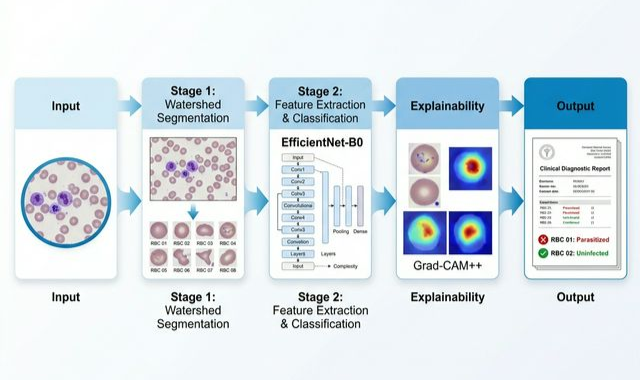
\includegraphics[width=\linewidth]{system_diagram_v1.png}
  \caption{\malariai{} two-stage decoupled architecture. Stage~1 performs
    universal cell segmentation via distance-transform guided watershed on the raw 1600$\times$1200
    blood smear image with no annotation input. Stage~2 classifies
    each 64$\times$64 crop with EfficientNet-B0 and Focal Loss,
    followed by Grad-CAM\texttt{++} for per-cell spatial explainability.}
  \label{fig:architecture}
\end{figure*}

\subsection{Dataset and Experimental Setup}
\label{ssec:dataset}

\paragraph{Dataset.}
All experiments use the NIH BBBC041 benchmark~\cite{bbbc041}, a publicly
available collection of Giemsa-stained thin \textit{Plasmodium falciparum}
blood smear images acquired at $100\times$ oil-immersion magnification.
The dataset comprises 1,208 training images and 120 held-out test images,
each at $1{,}600 \times 1{,}200$ pixels (RGB). Raw annotations total
80,113 bounding boxes in training and 5,922 in testing across seven
categories. Following standard practice, \textit{difficult} annotations
(441 training; 5 test) are excluded from all evaluations, yielding 79,672
and 5,917 valid boxes respectively.

\paragraph{Class distribution and imbalance.}
Table~\ref{tab:class_dist} and Figure~\ref{fig:class_dist} report per-class
annotation counts. The distribution is severely imbalanced: red blood cells
constitute 97.2\% of training annotations, while gametocytes account for
only 0.18\% --- a ratio of 537:1. A model predicting \textit{red blood cell}
for every instance achieves 97.2\% accuracy while detecting zero parasites.
This motivates Focal Loss~\cite{lin2017focal} with per-class inverse
frequency weights in Stage~2 (Section~\ref{ssec:stage2}).

\begin{table}[H]
\centering
\small
\caption{Per-class annotation counts in NIH BBBC041
  (\textit{difficult} annotations excluded).}
\label{tab:class_dist}
\renewcommand{\arraystretch}{1.15}
\begin{tabular}{lrrl}
\toprule
\textbf{Class} & \textbf{Train} & \textbf{Test} & \textbf{\% of Train} \\
\midrule
Red blood cell  & 77{,}420 & 5{,}614 & 97.18\% \\
Trophozoite     &  1{,}473 &    111  &  1.85\% \\
Ring            &    353   &    169  &  0.44\% \\
Schizont        &    179   &     11  &  0.22\% \\
Gametocyte      &    144   &     12  &  0.18\% \\
Leukocyte       &    103   &      0  &  0.13\% \\
\midrule
\textbf{Total}  & 79{,}672 &  5{,}917 & \\
\bottomrule
\end{tabular}
\end{table}

\begin{figure*}[t]
  \centering
  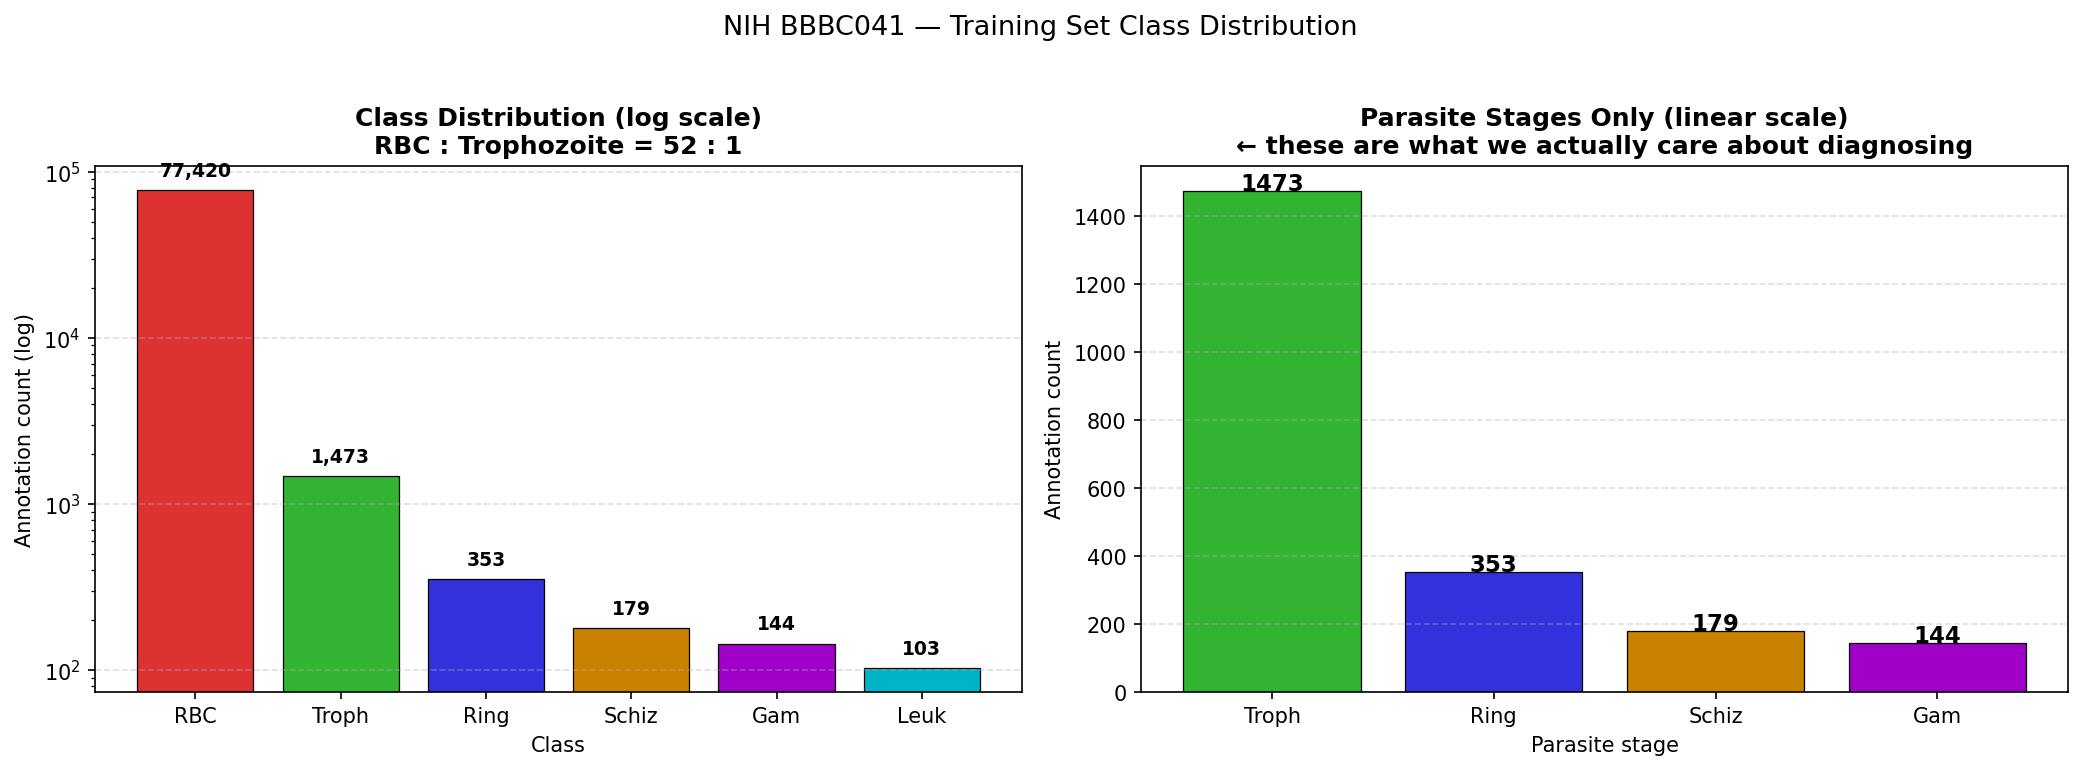
\includegraphics[width=\linewidth]{fig_class_distribution.png}
  \caption{Class distribution of NIH BBBC041 training annotations.
    Left: log-scale view dominated by the red blood cell class (77,420
    instances). Right: linear-scale view of parasitic stages only, showing
    the secondary imbalance between trophozoites (1,473) and the rarest
    stages (gametocyte: 144). The 537:1 RBC-to-gametocyte ratio motivates
    per-class Focal Loss weighting.}
  \label{fig:class_dist}
\end{figure*}

\paragraph{Parasitic stage morphology.}
Figure~\ref{fig:parasite_crops} shows representative crops for each
parasitic stage. Ring-stage infections present as pale discs with only a
faint peripheral chromatin outline, closely resembling uninfected RBCs.
Trophozoites exhibit irregular chromatin mass; schizonts show clear
internal segmentation (merozoites); gametocytes appear as large, densely
stained elongated bodies. This morphological hierarchy directly predicts
which classes the Stage~2 classifier will find most challenging.

\begin{figure*}[t]
  \centering
  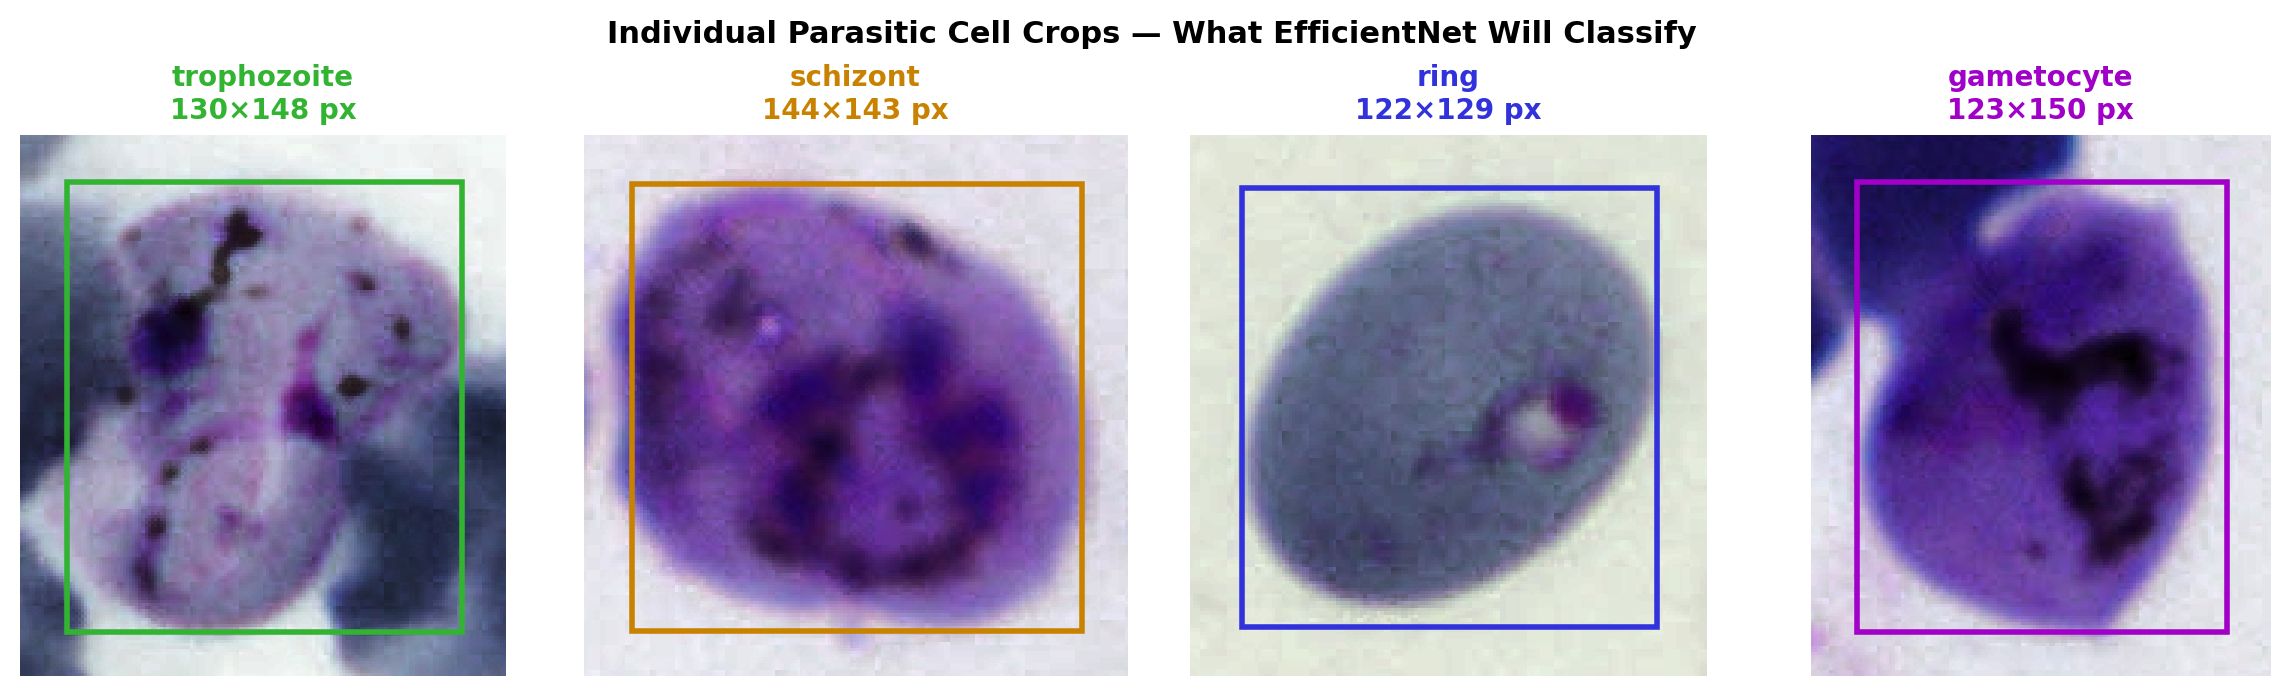
\includegraphics[width=\linewidth]{fig_parasite_crops.png}
  \caption{Representative ground-truth crops of each parasitic stage in
    NIH BBBC041 at native resolution. Ring-stage infections are visually
    the most similar to healthy RBCs, predicting lower per-class accuracy
    for that class. Parasitic stages are systematically larger than healthy
    erythrocytes (trophozoite median area: 17,272\,px$^2$; RBC: 11,544\,px$^2$),
    consistent with intraerythrocytic swelling during parasite development.}
  \label{fig:parasite_crops}
\end{figure*}

\paragraph{Annotation density and cell overlap.}
Figure~\ref{fig:density} shows the distribution of annotated boxes per
image. Density ranges from 9 to 223 boxes, with a median of 59 and a
95th percentile of 137; 11\% of images exceed 100 cells. To quantify
Problem~P2, we computed pairwise IoU between all ground-truth boxes within
each image over a 200-image sample. \textbf{58\%} of images contain at
least one ground-truth pair with $\text{IoU} > 0.3$, confirming that cell
overlap is a structural feature of the data. This empirical finding
directly motivates distance-transform watershed as Stage~1.

\begin{figure}[H]
  \centering
  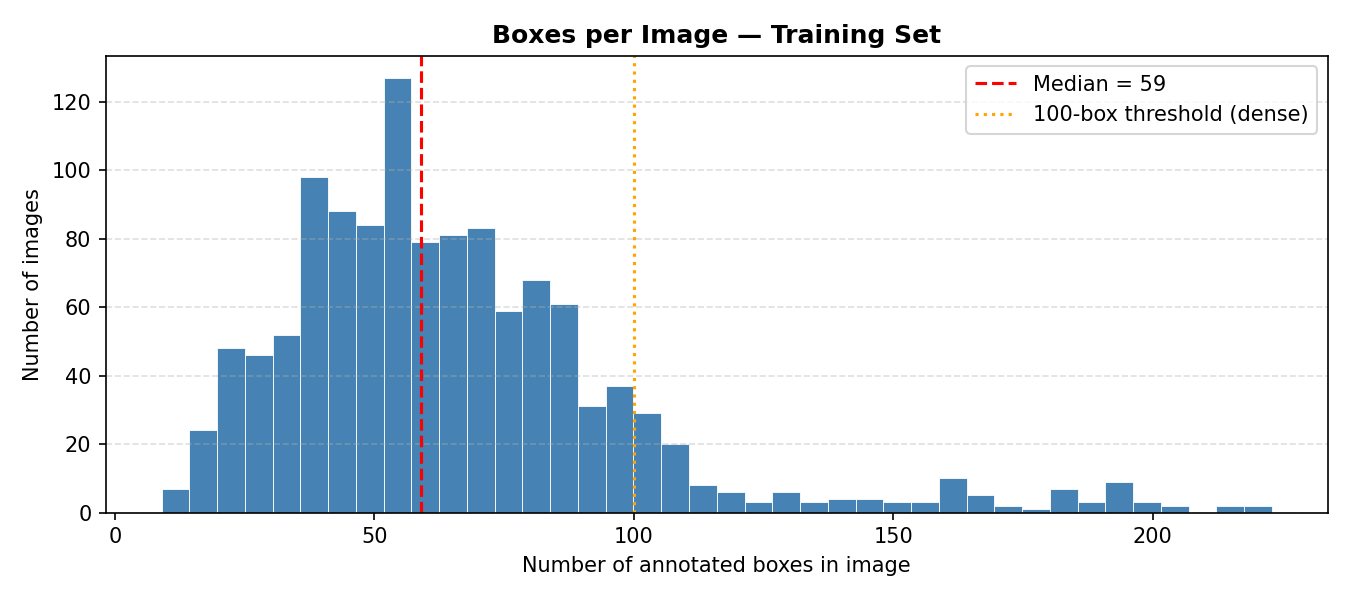
\includegraphics[width=\linewidth]{fig_density.png}
  \caption{Distribution of annotated bounding boxes per image in the
    BBBC041 training set (1,208 images). The dashed red line marks the
    median (59 boxes); the dotted orange line at 100 boxes identifies
    images we classify as \emph{dense smears}. 11\% of images exceed
    this threshold. 58\% of a 200-image sample contain at least one
    overlapping cell pair ($\text{IoU}>0.3$), confirming the severity of
    the NMS failure mode.}
  \label{fig:density}
\end{figure}

\paragraph{Train/validation/test protocol.}
The 1,208 training images are partitioned 80/20 at the image level into
training (966 images) and validation (242 images) splits. No image
contributes boxes to both sets. The random seed is fixed at 42 for
reproducibility. All hyperparameter decisions use the validation split
exclusively. The 120 test images are held out for Stage~1 evaluation only.

%% ----------------------------------------------------------------------------
\subsection{Cross-Dataset Validation: The MP-IDB Dataset}
\label{ssec:mpidb}

To assess generalisation beyond the NIH BBBC041 benchmark, we adopt the
\textit{Malaria Parasite Image Database} (MP-IDB)~\cite{delgado2020}
as a held-out cross-dataset evaluation set. MP-IDB comprises 209~images
from 17~distinct patient samples, acquired at 2{,}592$\times$1{,}944
pixels under Giemsa thin-smear staining --- the same staining protocol as
BBBC041, but a different institution, magnification calibration, and
patient cohort. Annotations were released in Supervisely bitmap-mask
format; we decode each mask via base64~$\rightarrow$~zlib~$\rightarrow$~PNG
and derive tight bounding boxes from the mask origin and dimensions,
yielding 1{,}407 annotated infected cells (script: \texttt{data/prepare\_mpidb.py}).

\paragraph{Taxonomy mismatch.}
MP-IDB labels cells at the \textit{species} level
(\textit{P.\ falciparum}, \textit{P.\ vivax}, \textit{P.\ malariae},
\textit{P.\ ovale}), whereas BBBC041 labels cells at the \textit{lifecycle
stage} level (ring, trophozoite, schizont, gametocyte). These taxonomies
are orthogonal: species identity does not determine lifecycle stage.
Accordingly, MP-IDB evaluation is \textit{binary}: any annotated object
is an infected cell (positive), and the pipeline's task is to detect it
regardless of species or stage.

\paragraph{Species and stage distribution.}
Figure~\ref{fig:mpidb_class_dist} shows the species breakdown.
\textit{P.\ falciparum} dominates (1{,}267 cells, 90.0\%), reflecting its
prevalence in clinical thin-smear datasets globally. Figure~\ref{fig:mpidb_stage_tags}
reports image-level lifecycle stage tags (multi-label): ring stage appears
in 125 images~(60\%), trophozoite in 54~(26\%), schizont in 38~(18\%),
and gametocyte in 26~(12\%), providing cross-stage diversity despite the
species-only annotation granularity.

\begin{figure*}[t]
  \centering
  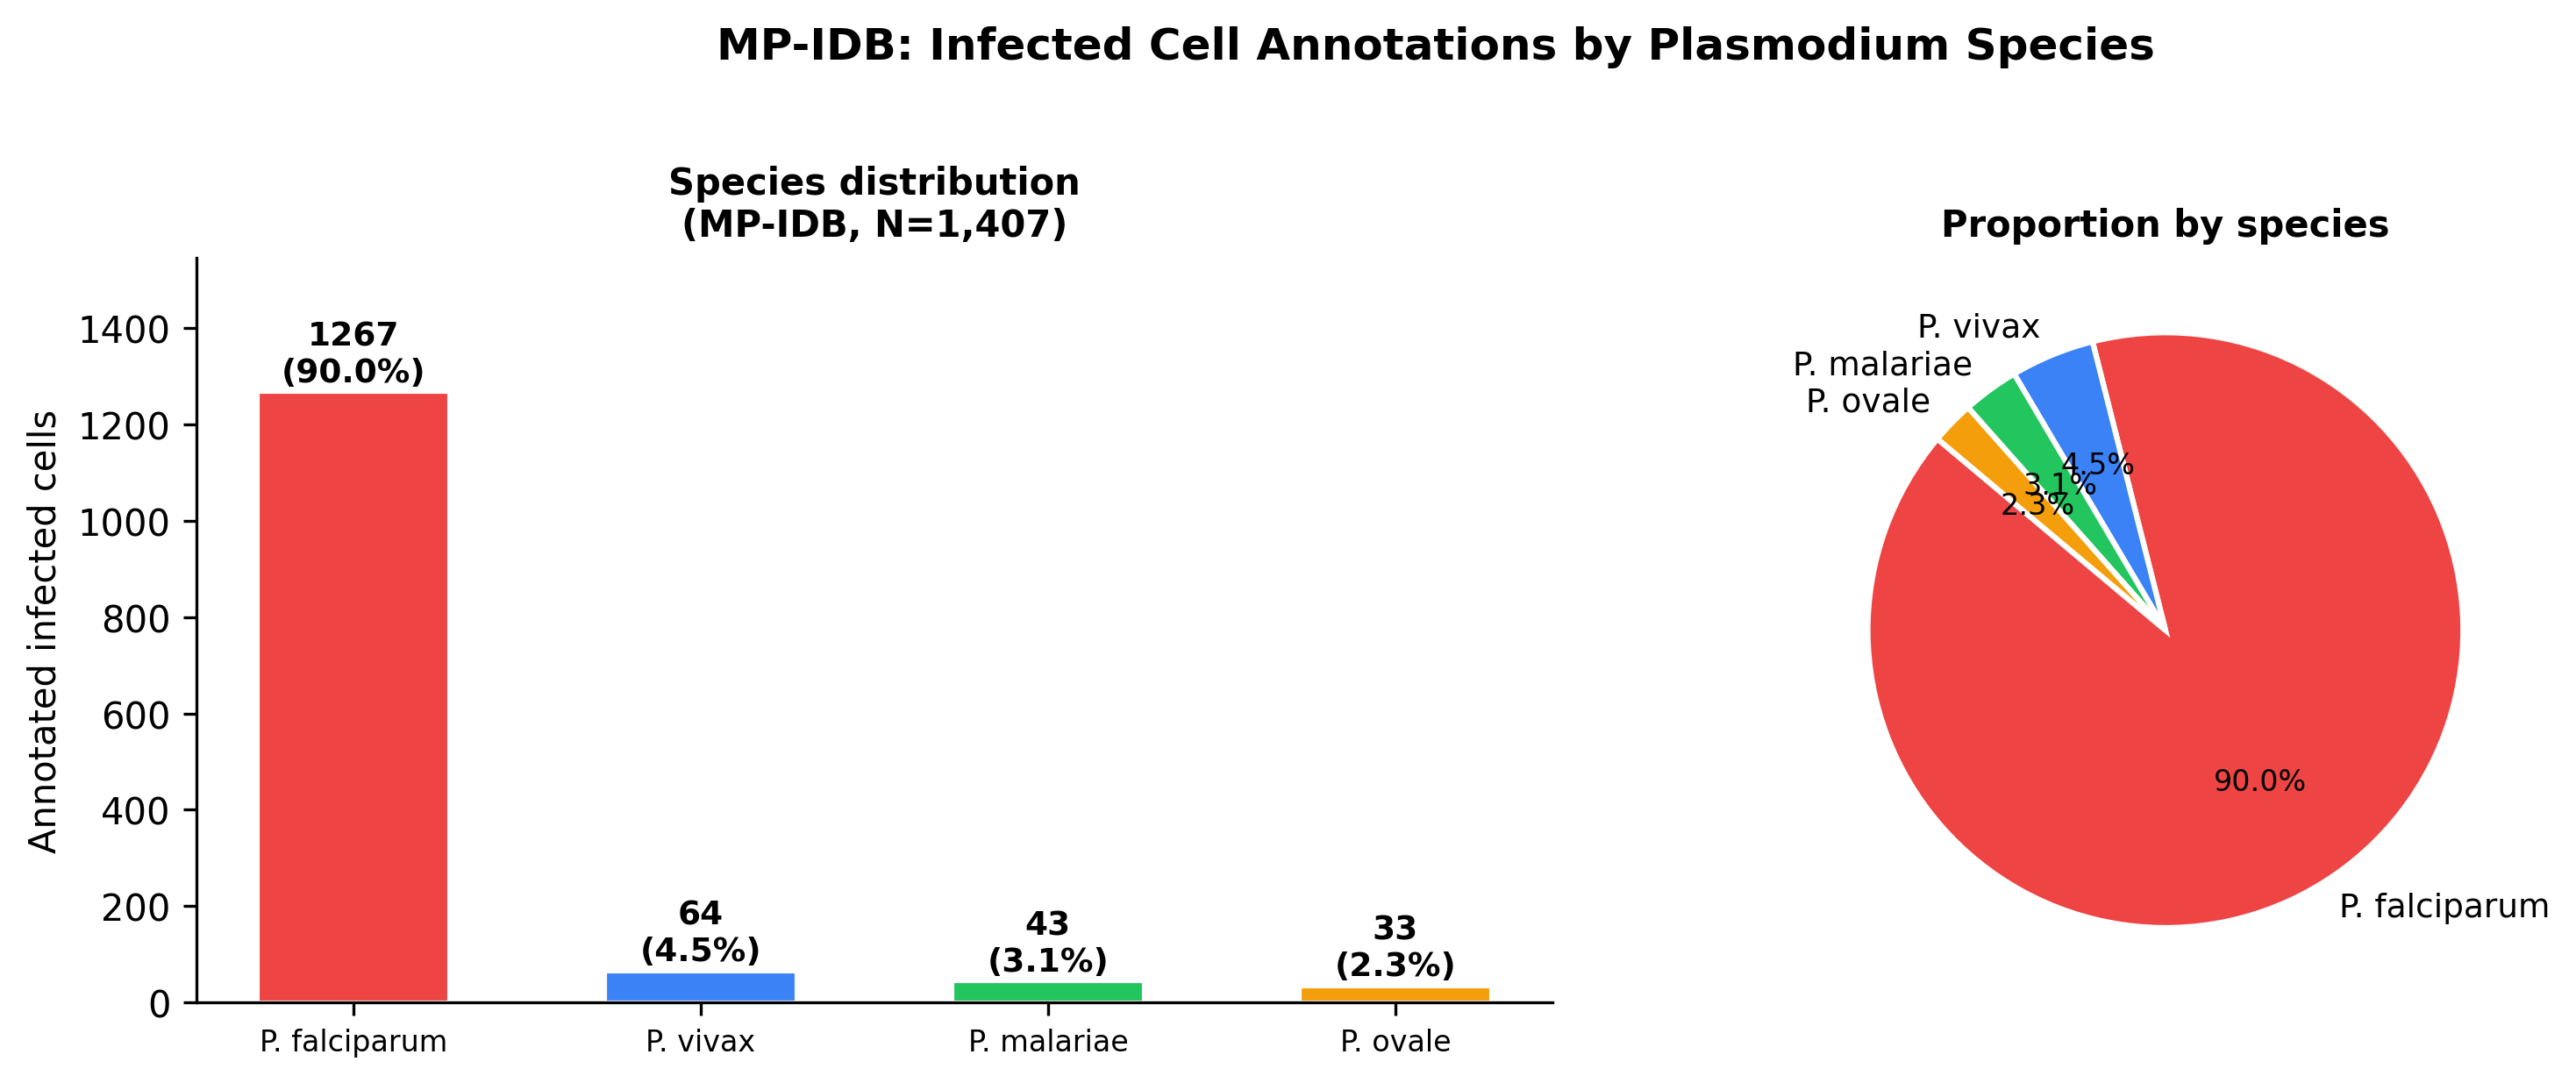
\includegraphics[width=\linewidth]{fig_mpidb_class_dist.png}
  \caption{MP-IDB species distribution. Left: annotation counts per
    \textit{Plasmodium} species across 209 images.
    \textit{P.\ falciparum} comprises 90.0\% of all annotated infected
    cells (1{,}267 of 1{,}407), consistent with its epidemiological
    prevalence. Right: proportional breakdown. The severe species imbalance
    mirrors the stage imbalance in BBBC041 and motivates binary (infected
    vs.\ uninfected) cross-dataset evaluation.}
  \label{fig:mpidb_class_dist}
\end{figure*}

\begin{figure}[H]
  \centering
  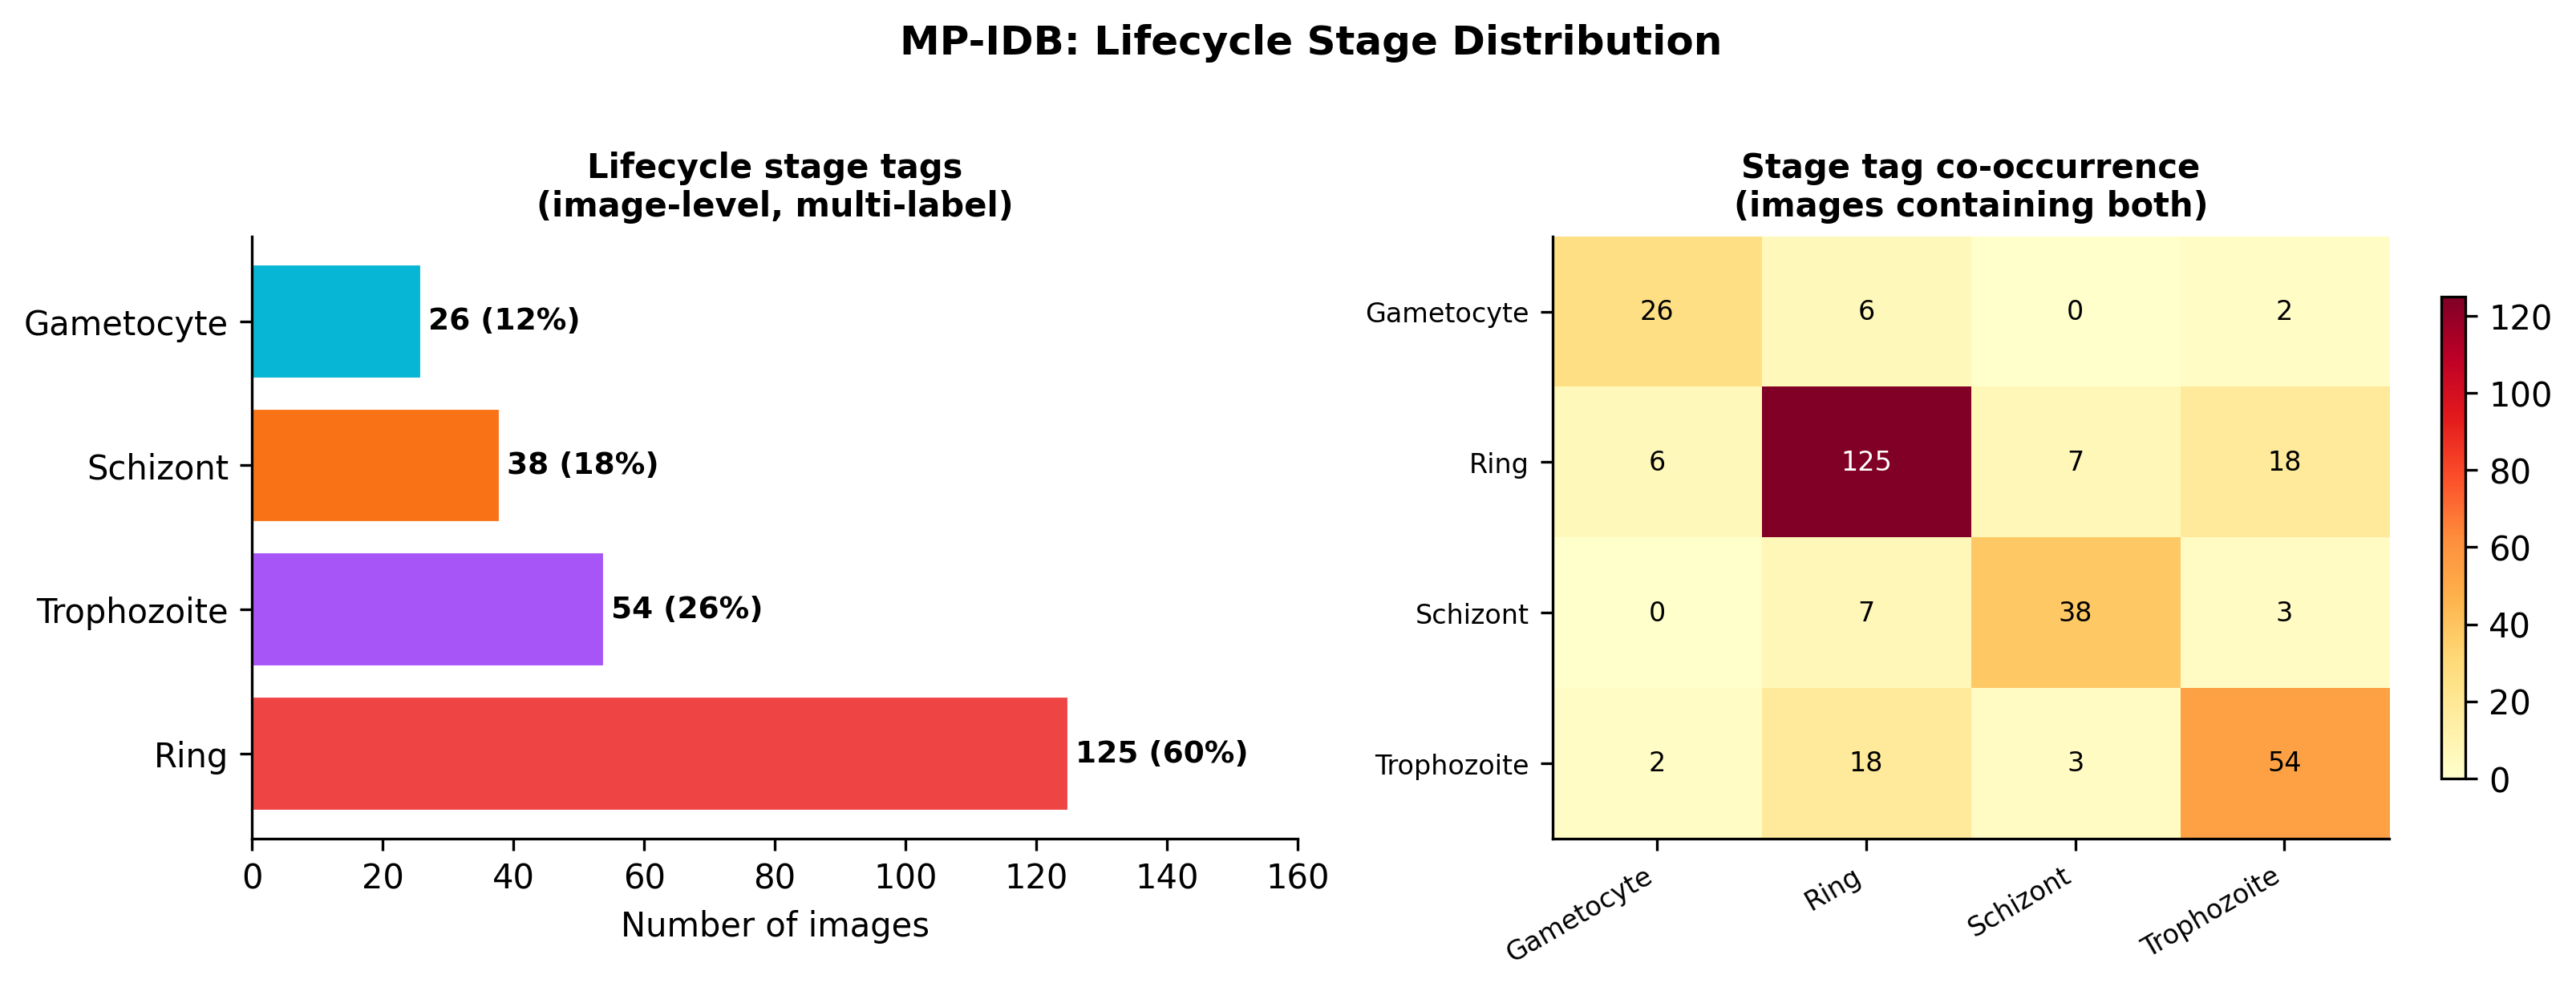
\includegraphics[width=\linewidth]{fig_mpidb_stage_tags.png}
  \caption{MP-IDB lifecycle stage distribution. Left: number of images
    containing each stage tag (multi-label; one image may carry multiple
    tags). Ring-stage infections are the most common (60\% of images).
    Right: tag co-occurrence matrix --- the 18 images tagged with both ring
    and trophozoite indicate mixed-stage smears, reflecting real clinical
    variability. Stage tags are image-level only; individual infected cells
    are not labelled by stage.}
  \label{fig:mpidb_stage_tags}
\end{figure}

\paragraph{Resolution and scale gap.}
A critical difference from BBBC041 is the bounding-box area of infected
cells. Figure~\ref{fig:mpidb_cell_size} shows that the median infected-cell
area in MP-IDB is 3{,}933\,px$^2$, compared with 16{,}875\,px$^2$ for
parasitic-stage cells in BBBC041 --- a 4.3$\times$ reduction in absolute
size. This is not a biological difference: cells are the same physical
size in both datasets. Rather, it reflects a difference in pixel density
per cell: MP-IDB images contain 2.63$\times$ more pixels overall
(5.04\,Mpx vs.\ 1.92\,Mpx) but fewer magnification-normalised pixels per
cell, so each infected cell covers only 0.078\% of the image frame versus
0.879\% in BBBC041 --- an 11.3$\times$ reduction in relative prominence.
Figure~\ref{fig:mpidb_scale_gap} illustrates this geometrically.

This scale gap has a direct consequence for Stage~1: the watershed
hyperparameters \texttt{MIN\_DIST}~$= 12$\,px and \texttt{MIN\_AREA}~$=
150$\,px$^2$ were tuned on BBBC041. For MP-IDB, the resolution-corrected
\texttt{MIN\_DIST} is approximately 20\,px, and the characteristic
infected-cell radius is only 35\,px versus 73\,px in BBBC041. Cross-dataset
evaluation on MP-IDB therefore provides an \emph{honest} assessment of
the pipeline's out-of-distribution behaviour without any parameter
re-tuning, and simultaneously motivates the Stage~1 adaptive improvements
described in future work (Section~\ref{ssec:limits}).

\begin{figure*}[t]
  \centering
  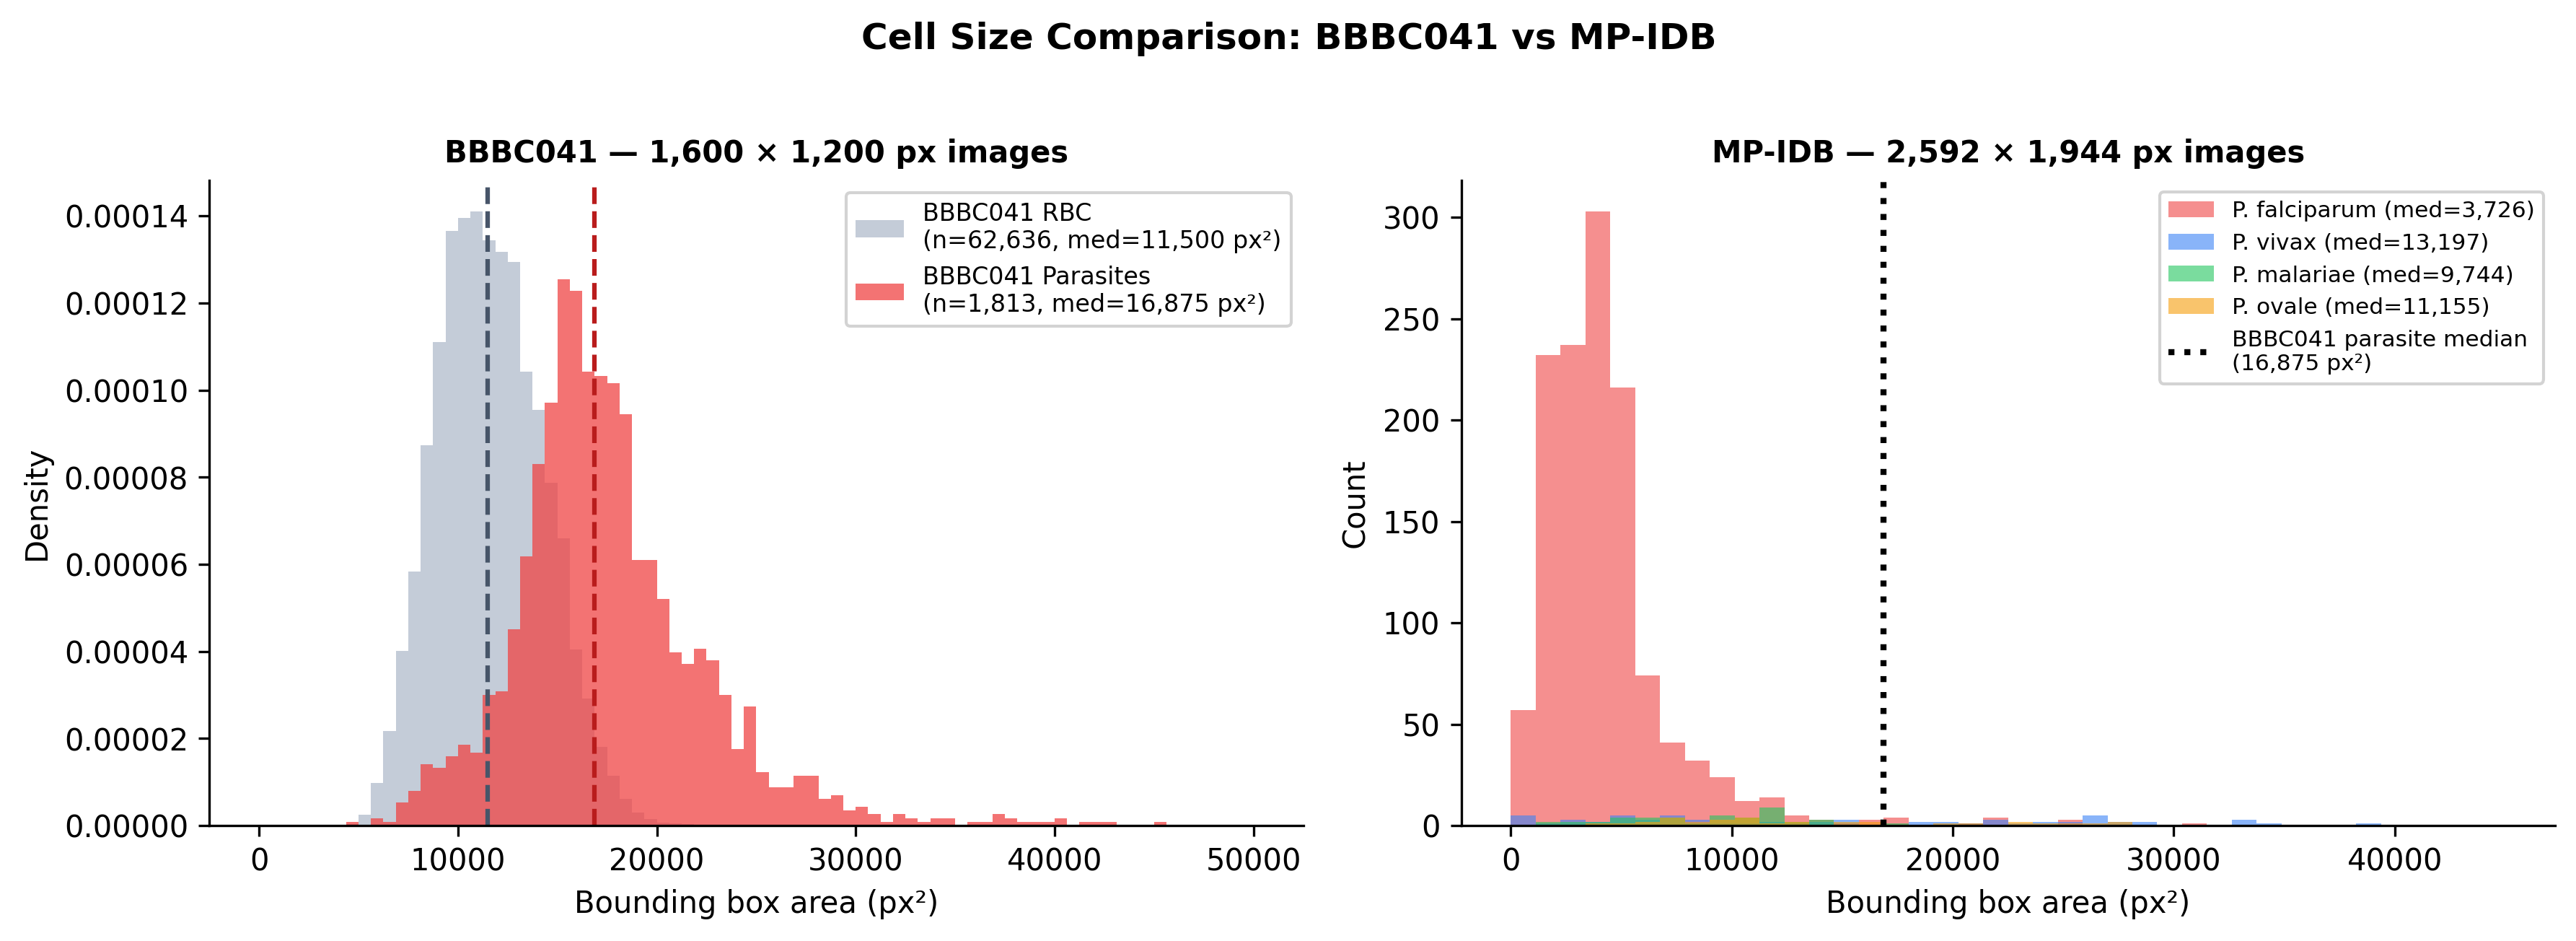
\includegraphics[width=\linewidth]{fig_mpidb_cell_size.png}
  \caption{Bounding-box area distributions for BBBC041 (left) and MP-IDB
    (right). Left: BBBC041 RBC and parasite distributions overlap
    substantially; the parasite median (16{,}875\,px$^2$) lies
    well above the RBC median (11{,}500\,px$^2$), reflecting intraerythrocytic
    swelling during parasite development. Right: MP-IDB infected-cell areas
    cluster at far lower values (median 3{,}933\,px$^2$ for
    \textit{P.\ falciparum}), 4.3$\times$ smaller than the BBBC041
    parasite median (dotted line). \textit{P.\ vivax} and \textit{P.\ ovale}
    show larger median areas (13{,}197 and 11{,}155\,px$^2$ respectively),
    consistent with their known tendency to infect larger reticulocytes.
    This scale gap directly predicts reduced Stage~1 recall on MP-IDB without
    parameter re-tuning.}
  \label{fig:mpidb_cell_size}
\end{figure*}

\begin{figure}[H]
  \centering
  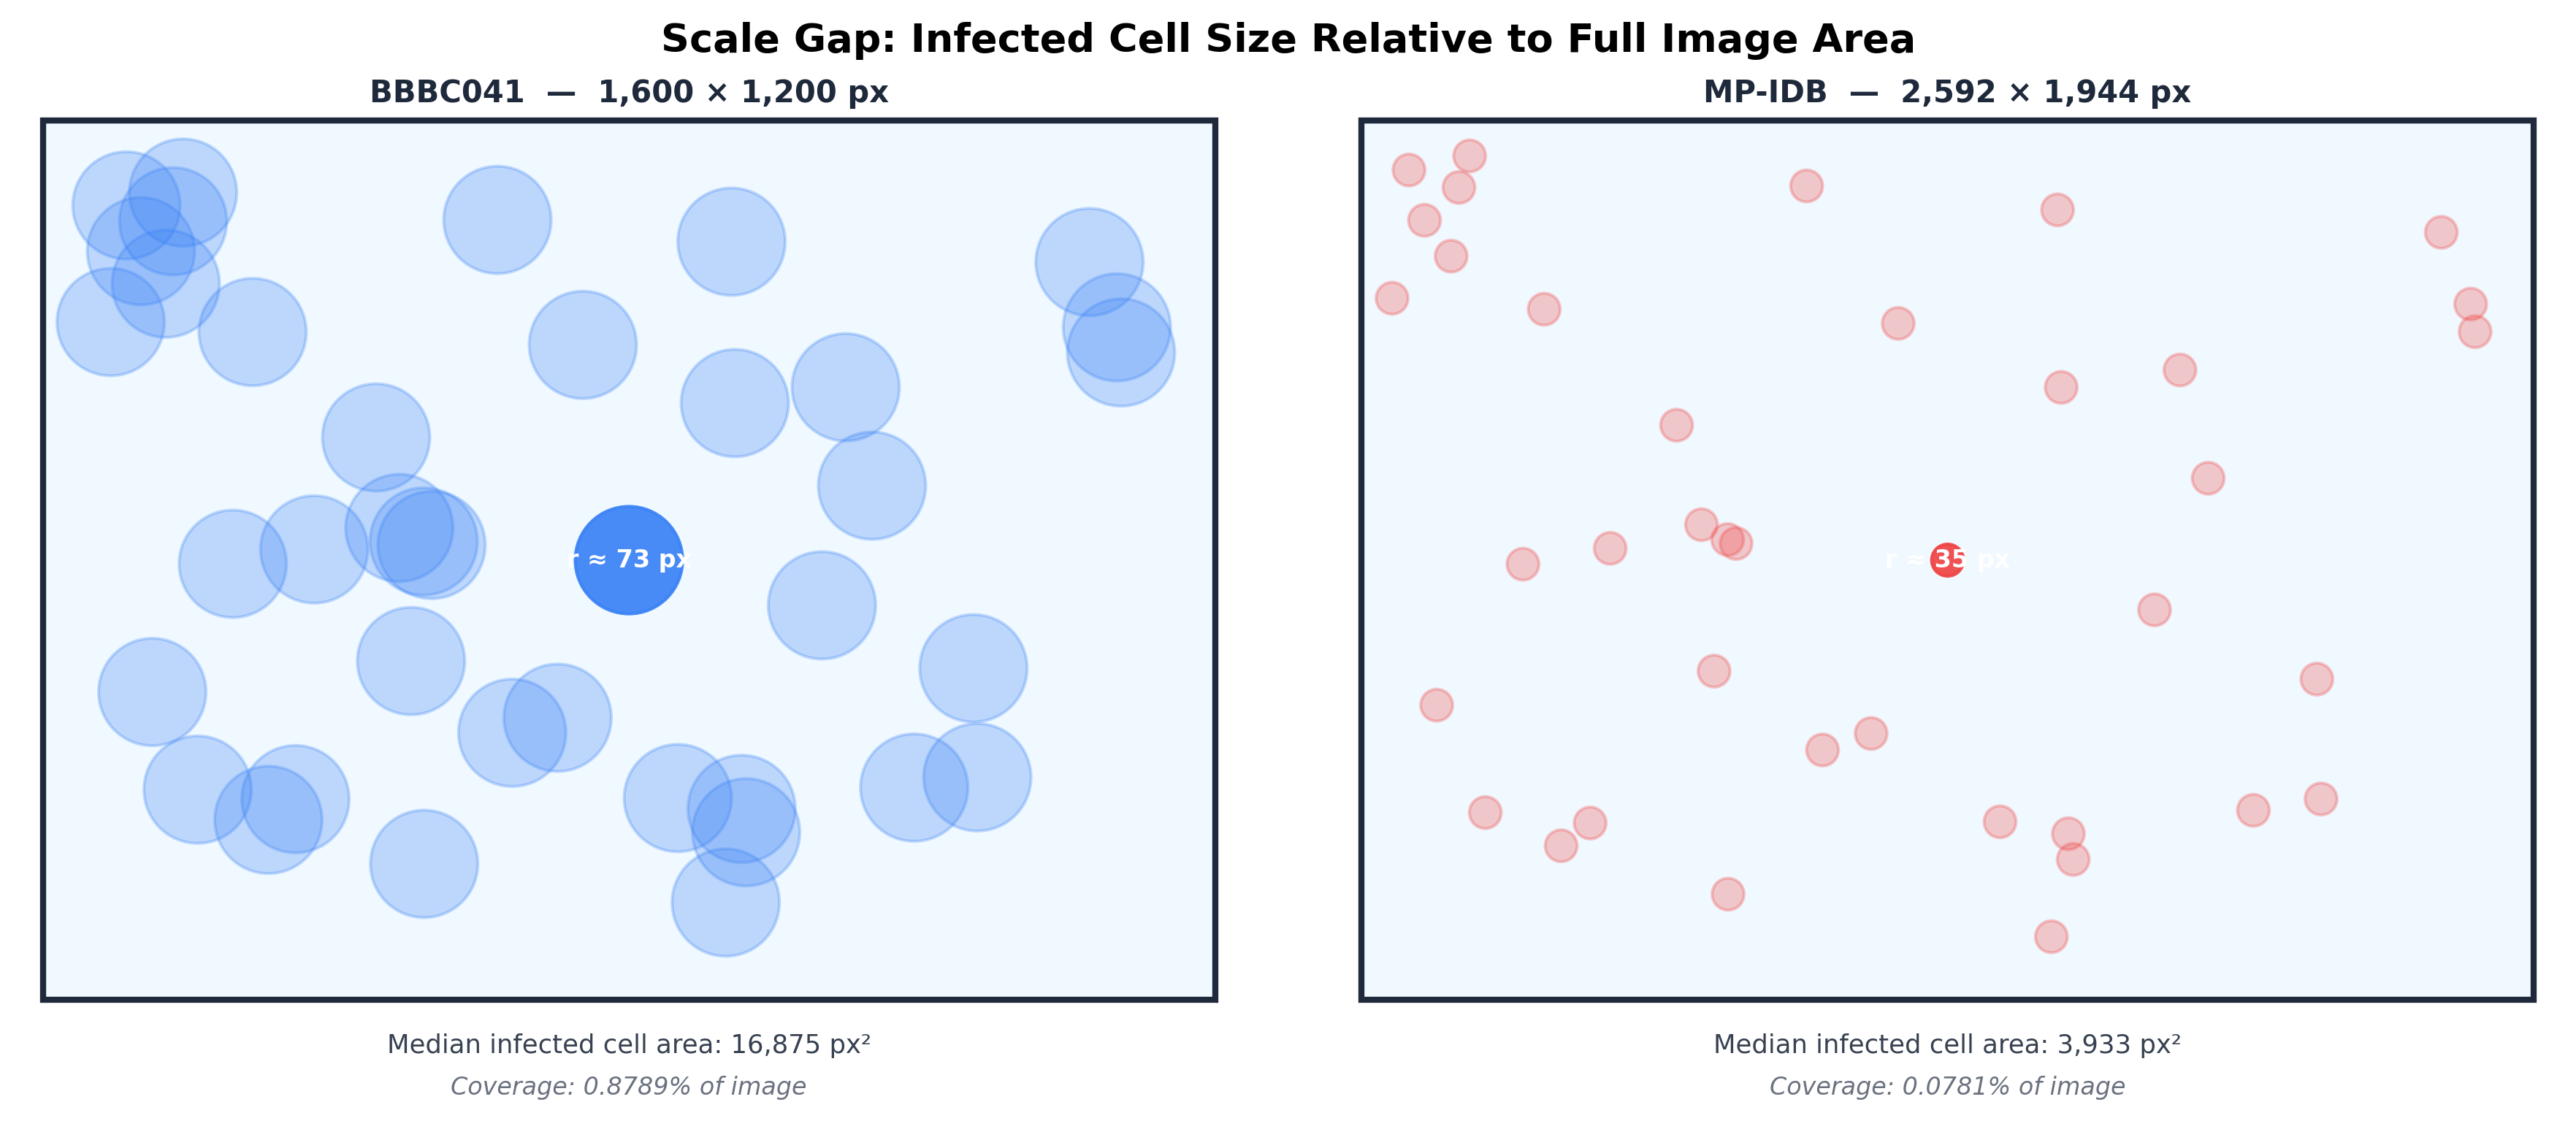
\includegraphics[width=\linewidth]{fig_mpidb_scale_gap.png}
  \caption{Geometric illustration of the scale gap between BBBC041 (left)
    and MP-IDB (right). Each circle represents an infected cell drawn to
    scale relative to the image frame. In BBBC041 the highlighted cell
    (radius $r \approx 73$\,px) covers 0.88\% of the image; in MP-IDB the
    corresponding cell (radius $r \approx 35$\,px) covers only 0.078\%.
    Watershed parameters tuned on BBBC041 underperform on MP-IDB without
    resolution-aware adaptation.}
  \label{fig:mpidb_scale_gap}
\end{figure}

\begin{figure*}[t]
  \centering
  \includegraphics[width=\linewidth]{fig_mpidb_samples.png}
  \caption{Representative MP-IDB images with ground-truth bounding boxes
    overlaid. Red boxes: \textit{P.\ falciparum}; blue: \textit{P.\ vivax};
    green: \textit{P.\ malariae}; yellow: \textit{P.\ ovale}. Images span
    multiple patients and lifecycle stages. The top row shows standard
    Giemsa staining; the bottom row shows images from a patient with slightly
    different background colouration, illustrating intra-cohort staining
    variability. Infected cells are visually subtle relative to the large
    number of healthy RBCs, confirming the detection challenge.}
  \label{fig:mpidb_samples}
\end{figure*}

Table~\ref{tab:dataset_comparison} summarises the key properties of both
datasets side by side.

\begin{table}[H]
\centering
\small
\caption{Comparison of primary (BBBC041) and cross-validation (MP-IDB) datasets.}
\label{tab:dataset_comparison}
\renewcommand{\arraystretch}{1.15}
\begin{tabular}{lll}
\toprule
\textbf{Property} & \textbf{BBBC041 (primary)} & \textbf{MP-IDB (cross-val)} \\
\midrule
Source              & NIH / Broad Institute     & Delgado-Ortet et al.\ (2020) \\
Images              & 1{,}328 (train + test)    & 209 (annotated) \\
Resolution          & 1{,}600$\times$1{,}200\,px  & 2{,}592$\times$1{,}944\,px \\
Image area          & 1.92\,Mpx                 & 5.04\,Mpx \\
Annotation type     & Bounding boxes            & Bitmap masks $\rightarrow$ boxes \\
Label taxonomy      & Stage-level               & Species-level \\
Infected cells      & 1{,}841                   & 1{,}407 \\
Healthy cells labelled & Yes (77{,}831 RBCs)   & No \\
Median cell area    & 16{,}875\,px$^2$          & 3{,}933\,px$^2$ \\
Cell image coverage & 0.879\%                   & 0.078\% \\
Patients            & Not reported              & 17 \\
Staining            & Giemsa thin smear         & Giemsa thin smear \\
\bottomrule
\end{tabular}
\end{table}

%% ----------------------------------------------------------------------------
\subsection{Stage 1: Universal Cell Segmentation}
\label{ssec:stage1}

Stage~1 applies a five-step computer vision pipeline to produce an ordered
set of bounding boxes $\mathcal{B} = \{(x_1^i, y_1^i, x_2^i, y_2^i)\}_{i=1}^N$
from a raw blood smear image $\mathbf{I} \in \mathbb{R}^{H \times W \times 3}$,
where $N$ is determined entirely by the image content and no ground-truth
annotation is consulted at any step.

\paragraph{Step 1 --- Grayscale conversion and Otsu thresholding.}
The input BGR image is converted to a single-channel grayscale image
$G \in \mathbb{R}^{H \times W}$ using the standard luminosity transform.
Otsu's method~\cite{otsu1979} selects the threshold $\tau^*$ that maximises
inter-class variance between foreground (cells) and background:

\begin{equation}
  \tau^* = \arg\max_\tau \; \omega_0(\tau)\,\omega_1(\tau)\,
  \bigl[\mu_0(\tau) - \mu_1(\tau)\bigr]^2
  \label{eq:otsu}
\end{equation}

where $\omega_k$ and $\mu_k$ are the prior probability and mean grey level
of class $k$. The binary mask is formed as $B = \mathbf{1}[G < \tau^*]$
(inverse: cells are dark, background is bright in Giemsa-stained smears),
so foreground pixels take value 255 and background pixels take 0.

\paragraph{Step 2 --- Morphological opening.}
A morphological opening with a $3 \times 3$ elliptical structuring element
applied for two iterations removes thin noise filaments from the binary
mask while preserving cell bodies:

\begin{equation}
  O = (B \ominus K) \oplus K
  \label{eq:open}
\end{equation}

where $\ominus$ denotes erosion and $\oplus$ denotes dilation. The small
kernel size (3\,px) is chosen to minimise erosion of cell boundaries,
which is important for accurately locating watershed seeds at cell centres.

\paragraph{Step 3 --- Euclidean distance transform.}
The Euclidean distance transform $D$ assigns to each foreground pixel
$(x,y)$ its minimum distance to any background pixel:

\begin{equation}
  D(x,y) = \min_{(p,q) \notin O} \sqrt{(x-p)^2 + (y-q)^2}
  \label{eq:dist}
\end{equation}

Peaks in $D$ correspond to cell centres: a pixel at the centre of a
perfectly circular cell of radius $r$ achieves $D = r$, while pixels
near the boundary achieve $D \approx 0$. In dense regions, the distance
transform naturally produces a ridge between adjacent cells, creating
the topological separator that watershed uses for instance-level splitting.

\paragraph{Step 4 --- Seed extraction via local maxima.}
Seeds for the watershed algorithm are extracted as local maxima of $D$
that satisfy two conditions: (i) they are separated by at least
\texttt{MIN\_DIST}~$= 12$ pixels from any higher-valued maximum, and
(ii) they exceed an absolute threshold $\tau_{\text{seed}} = 0.25 \times D_{\max}$.
The minimum distance of 12\,px (compared to the typical RBC radius of
$\sim$50\,px) ensures one seed per cell without suppressing seeds in
adjacent cells. The distance threshold of 0.25 places seeds only at
genuine cell centres, not at shallow bumps caused by staining artefacts.

\paragraph{Step 5 --- Watershed segmentation and bounding box extraction.}
Seeds are labelled as independent markers and watershed is applied to the
negated distance map $-D$ with the binary mask $O$ as the allowed domain:

\begin{equation}
  \mathcal{L} = \text{watershed}(-D,\; \text{markers},\; \text{mask}=O)
  \label{eq:watershed}
\end{equation}

Each labelled region $\ell$ in $\mathcal{L}$ yields a bounding box
$(x_1, y_1, x_2, y_2)$ from the extreme pixel coordinates of that region.
Regions with fewer than \texttt{MIN\_AREA}~$= 150$ pixels are discarded
as noise. A compactness parameter of 0.1 regularises elongated regions
produced by connected cell clusters, biasing watershed boundaries toward
the topological saddle points in $D$.

Figure~\ref{fig:watershed_alg} summarises the complete Stage~1 procedure.

\begin{figure}[t]
\centering
\fbox{\begin{minipage}{0.92\linewidth}
\vspace{0.5em}
\small
\noindent\textbf{Algorithm 1:} Stage~1 --- Annotation-Agnostic Watershed Segmentation
\vspace{0.5em}

\noindent\textbf{Require:} Blood smear image $\mathbf{I} \in \mathbb{R}^{H \times W \times 3}$\\[0.2em]
\textbf{Ensure:} Bounding boxes $\mathcal{B} = \{(x_1^i, y_1^i, x_2^i, y_2^i)\}$
\vspace{0.4em}

\noindent
\begin{tabular}{@{\hspace{0.5em}}rl@{}}
1.  & $G \;\leftarrow\; \mathrm{BGR2GRAY}(\mathbf{I})$\\[3pt]
2.  & $\tau^* \;\leftarrow\; \mathrm{OtsuThreshold}(G)$\\[3pt]
3.  & $B \;\leftarrow\; \mathbf{1}[G < \tau^*]$ \quad \textit{// foreground = cells}\\[3pt]
4.  & $O \;\leftarrow\; \mathrm{MorphOpen}(B,\; k{=}3,\; \mathrm{iters}{=}2)$\\[3pt]
5.  & $D \;\leftarrow\; \mathrm{DistanceTransform}(O)$\\[3pt]
6.  & $\mathcal{S} \;\leftarrow\; \mathrm{LocalMaxima}(D,\; d_{\min}{=}12,\;
      \tau_{\mathrm{seed}}{=}0.25\,D_{\max})$\\[3pt]
7.  & $M \;\leftarrow\; \mathrm{LabelSeeds}(\mathcal{S})$\\[3pt]
8.  & $\mathcal{L} \;\leftarrow\; \mathrm{watershed}(-D,\; M,\; O)$;
      \quad $\mathcal{B} \;\leftarrow\; \emptyset$\\[3pt]
9.  & \textbf{for} each region $\ell \in \mathcal{L}$:
      \textbf{if} $|\ell| \geq 150$ \textbf{then}
      $\mathcal{B} \;\leftarrow\; \mathcal{B} \cup \{\mathrm{BBox}(\ell)\}$\\[3pt]
10. & \textbf{return} $\mathcal{B}$\\
\end{tabular}
\vspace{0.4em}
\end{minipage}}
\caption{Stage~1 annotation-agnostic watershed segmentation (Algorithm~1).
  Parameters: \texttt{MIN\_DIST}$\!=\!12$\,px, $\tau_{\mathrm{seed}}\!=\!0.25$,
  \texttt{MIN\_AREA}$\!=\!150$\,px$^2$.}
\label{fig:watershed_alg}
\end{figure}

\paragraph{Post-processing: oversized region filtering.}
In particularly dense regions where 3--5 cells are packed without any
visible inter-cell gap, the distance transform may not generate sufficient
seed separation to split the cluster. The resulting watershed region
spans the entire cluster and produces an oversized bounding box. Such
regions (width $> 220$\,px, height $> 220$\,px, or aspect ratio $> 2.2$)
are excluded from Stage~2 classification and flagged as ``merged cluster''
in the visual output. This prevents the EfficientNet classifier from
receiving a crop containing multiple cells --- an input it was not trained
on --- and avoids systematic misclassification of cluster crops as
leukocytes (the closest large-cell training class).

%% ----------------------------------------------------------------------------
\subsection{Stage 2: EfficientNet-B0 Classifier with Focal Loss}
\label{ssec:stage2}

\paragraph{Crop extraction.}
For each bounding box $(x_1, y_1, x_2, y_2) \in \mathcal{B}$ produced by
Stage~1, we extract a square crop centred on the box centroid. The crop
is resized to $64 \times 64$ pixels using bilinear interpolation. If the
centred crop extends beyond image boundaries, the image is reflect-padded
before extraction to avoid black border artefacts. The final crop is a
uint8 RGB array normalised to ImageNet statistics ($\mu = [0.485,\,0.456,\,0.406]$,
$\sigma = [0.229,\,0.224,\,0.225]$).

\paragraph{EfficientNet-B0 architecture.}
We use EfficientNet-B0~\cite{tan2019} as the Stage~2 classification
backbone. EfficientNet applies compound scaling --- simultaneously scaling
network depth, width, and input resolution by constants derived from a
neural architecture search --- to achieve better parameter efficiency than
models scaled along a single axis. EfficientNet-B0 is the baseline scaling
point ($d=1.0,\;w=1.0,\;r=224$) and has 5.3M parameters, making it
deployable for CPU inference without GPU infrastructure. The final
classification head (a single Linear layer) is replaced with
$\text{Linear}(1280, 7)$ to match the seven BBBC041 categories (six cell
classes plus background). The convolutional backbone is initialised from
ImageNet weights to leverage low-level texture features acquired during
pretraining.

\paragraph{Focal Loss with per-class inverse-frequency weighting.}
Standard cross-entropy loss applied to the 537:1 class-imbalanced BBBC041
distribution produces a degenerate solution: the model achieves high
accuracy by predicting \textit{red blood cell} for every crop. We address
this with Focal Loss~\cite{lin2017focal}, which down-weights the loss
contribution of easily classified examples:

\begin{equation}
  \mathcal{L}_{\text{focal}}(p_t) =
  -\alpha_t \,(1-p_t)^{\gamma}\,\log(p_t)
  \label{eq:focal}
\end{equation}

where $p_t$ is the model's estimated probability for the ground-truth class,
$\gamma = 2.0$ is the focusing parameter that reduces loss weight for
well-classified examples (those with $p_t \to 1$), and $\alpha_t$ is a
per-class weight. We set $\alpha_t$ by inverse-frequency normalisation:

\begin{equation}
  \alpha_c = \frac{1/n_c}{\max_{c'} \; 1/n_{c'}}
  \label{eq:alpha}
\end{equation}

where $n_c$ is the number of training crops for class $c$ and the maximum
is taken over all foreground classes. This assigns $\alpha = 1.0$ to the
rarest class (leukocyte: 103 instances) and proportionally lower weights
to more frequent classes ($\alpha_{\text{RBC}} \approx 0.0013$). The
background class receives $\alpha = 0$ and contributes no gradient.
Computed weights are summarised in Table~\ref{tab:focal_weights}.

\begin{table}[H]
\centering
\small
\caption{Per-class Focal Loss weights $\alpha_c$ computed from BBBC041
  training annotation counts via Equation~\ref{eq:alpha}.}
\label{tab:focal_weights}
\renewcommand{\arraystretch}{1.15}
\begin{tabular}{lrrr}
\toprule
\textbf{Class} & \textbf{Count} ($n_c$) & \textbf{$1/n_c$} & $\alpha_c$ \\
\midrule
Red blood cell  & 77,420 & $1.29 \times 10^{-5}$ & 0.0013 \\
Trophozoite     &  1,473 & $6.79 \times 10^{-4}$ & 0.0699 \\
Ring            &    353 & $2.83 \times 10^{-3}$ & 0.2918 \\
Schizont        &    179 & $5.59 \times 10^{-3}$ & 0.5754 \\
Gametocyte      &    144 & $6.94 \times 10^{-3}$ & 0.7153 \\
Leukocyte       &    103 & $9.71 \times 10^{-3}$ & 1.0000 \\
\bottomrule
\end{tabular}
\end{table}

\paragraph{Training details.}
The Stage~2 classifier is trained for 30 epochs on 79,672 pre-extracted
$64\times 64$ crops from the 966-image training split (one crop per
annotated bounding box). Pre-extraction --- saving all crops as PNG files
before training begins --- reduces the per-epoch I/O cost from loading
1,208 full 1600$\times$1200 images to loading 79,672 small crops,
reducing training time from $\sim$41 minutes per epoch to $\sim$50
seconds per epoch on an NVIDIA T4 GPU with batch size 128.

Training augmentation applied to each crop: random horizontal and vertical
flips (p = 0.5 each), ColorJitter with brightness $\pm 0.2$, contrast
$\pm 0.2$, and saturation $\pm 0.1$ to simulate staining variation across
laboratories. The AdamW optimiser ($lr = 3 \times 10^{-4}$,
weight decay $= 10^{-4}$) is paired with a CosineAnnealingLR schedule
(T\_max = 30, $\eta_{\min} = 10^{-6}$), smoothly decaying the learning
rate to near-zero by epoch 30 and avoiding the abrupt validation loss
increase we observe in Baseline A when step-decay is applied. The best
checkpoint is selected by maximum validation accuracy.

%% ----------------------------------------------------------------------------
\subsection{Grad-CAM\texttt{++} Explainability}
\label{ssec:gradcam}

\paragraph{Motivation for Grad-CAM\texttt{++} over Grad-CAM.}
Standard Grad-CAM~\cite{selvaraju2017} weights each spatial activation
map by the global average of its gradients with respect to the target class
score. This approach suffers from single-activation bias: when multiple
spatial locations jointly contribute to the classification (common in
small $64 \times 64$ crops where the parasite occupies most of the
receptive field), Grad-CAM over-attributes saliency to the location with
the highest single gradient value. Grad-CAM\texttt{++}~\cite{chattopadhyay2018}
addresses this with second- and third-order gradient terms that assign
more accurate per-location attribution weights.

\paragraph{Mathematical formulation.}
Let $A^k \in \mathbb{R}^{h \times w}$ denote the feature map of the
$k$-th channel at the target convolutional layer, and let $S^c$ be the
score for target class $c$ before softmax. The Grad-CAM\texttt{++} weight
for channel $k$ is:

\begin{equation}
  w_k^c = \sum_{i,j} \alpha_{kij}^c \cdot \text{ReLU}
  \!\left(\frac{\partial S^c}{\partial A_{ij}^k}\right)
  \label{eq:gcampp_weight}
\end{equation}

where the pixel-wise coefficient $\alpha_{kij}^c$ is:

\begin{equation}
  \alpha_{kij}^c = \frac{
    \left(\dfrac{\partial^2 S^c}{\partial (A_{ij}^k)^2}\right)
  }{
    2\,\dfrac{\partial^2 S^c}{\partial (A_{ij}^k)^2}
    + \displaystyle\sum_{a,b} A_{ab}^k \cdot
    \dfrac{\partial^3 S^c}{\partial (A_{ij}^k)^3} + \varepsilon
  }
  \label{eq:alpha_gcam}
\end{equation}

In practice, denoting first-, second-, and third-order gradient tensors
as $G^{(1)} = \partial S^c / \partial A^k$, $G^{(2)} = (G^{(1)})^2$,
and $G^{(3)} = (G^{(1)})^3$, Equation~\ref{eq:alpha_gcam} becomes:

\begin{equation}
  \alpha^c = \frac{G^{(2)}}{2\,G^{(2)}
  + \bigl(A \cdot G^{(3)}\bigr)_{\text{sum}} + \varepsilon}
  \label{eq:alpha_gcam_compact}
\end{equation}

The final heatmap is:

\begin{equation}
  L^c_{\text{Grad-CAM++}} = \text{ReLU}
  \!\left(\sum_k w_k^c \cdot A^k\right)
  \label{eq:gcampp_cam}
\end{equation}

upsampled bilinearly to the input resolution ($64 \times 64$) and
normalised to $[0, 1]$.

\paragraph{Hook target.}
Hooks are registered on \texttt{model.features[-1]}, the final MBConv
block of EfficientNet-B0, producing feature maps of shape $[B, 1280, 2, 2]$
for $64\times 64$ inputs. This layer has a receptive field spanning most
of the crop, making it the most informative layer for attribution.

\paragraph{Output views.}
Two visualisations are produced per blood smear:
(i) a \textit{Grad-CAM\texttt{++} crop gallery} showing each detected
parasite as a 160$\times$160 pixel overlay of the original crop and
heatmap (jet colourmap, $\alpha = 0.5$), labelled with class name and
confidence; and
(ii) a \textit{full-image Grad-CAM\texttt{++} overlay} that splats each
parasite's heatmap back onto the full 1600$\times$1200 smear at the
bounding box coordinates, using a spatial mask so only parasite-detected
regions are heatmap-coloured and the remainder of the image is unchanged.

%% ----------------------------------------------------------------------------
\subsection{Baseline A: Faster R-CNN}
\label{ssec:baseline}

Pipeline A is a Faster R-CNN~\cite{ren2015} with a ResNet-50 Feature
Pyramid Network (FPN) backbone pretrained on MS-COCO. The standard 91-class
classification head is replaced with a 7-class \texttt{FastRCNNPredictor}.
The FPN generates multi-scale feature maps at strides \{4, 8, 16, 32, 64\},
enabling detection of both large cells (\eg, leukocytes, median area
$\approx$14,000\,px$^2$) and small ring-stage nuclei ($\approx$3,500\,px$^2$).

\paragraph{Training protocol.}
The model is trained for 80 epochs on the 966-image training split using
SGD ($lr = 5 \times 10^{-3}$, momentum $= 0.9$, weight decay $= 10^{-4}$)
with a MultiStepLR schedule ($\gamma = 0.1$ at epoch 50) and gradient
clipping (max norm 10.0). Batch size 4 on an NVIDIA T4 GPU. Best checkpoint
selected by minimum validation loss.

\paragraph{Structural training ceiling.}
Figure~\ref{fig:frcnn_loss} shows the training and validation loss curves.
Validation loss plateaus at $\approx 0.23$ from epoch~8, while training
loss continues to fall. After the learning rate drop at epoch~50, training
loss decreases to 0.08 while validation loss \emph{increases} to 0.28.
This divergence begins before any opportunity for conventional overfitting
and is the empirical signature of Problem~P1: the model correctly detects
unannotated cells but is penalised by the closed-world loss function. The
best checkpoint is epoch~23 (val.\ loss 0.2294); 57 subsequent epochs
produce no improvement.

\begin{figure}[H]
  \centering
  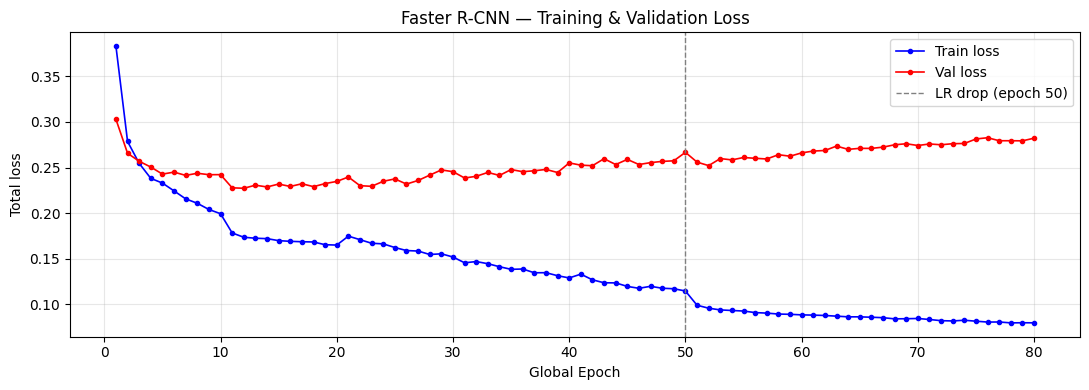
\includegraphics[width=\linewidth]{fig_frcnn_loss.png}
  \caption{Faster R-CNN (Baseline A) training and validation loss over
    80 epochs. Validation loss plateaus at $\approx 0.23$ from epoch~8
    and increases after the learning rate drop at epoch~50 --- the
    empirical signature of annotation incompleteness (Problem~P1).
    Best checkpoint: epoch~23 (val.\ loss 0.2294).}
  \label{fig:frcnn_loss}
\end{figure}

\begin{figure}[t]
  \centering
  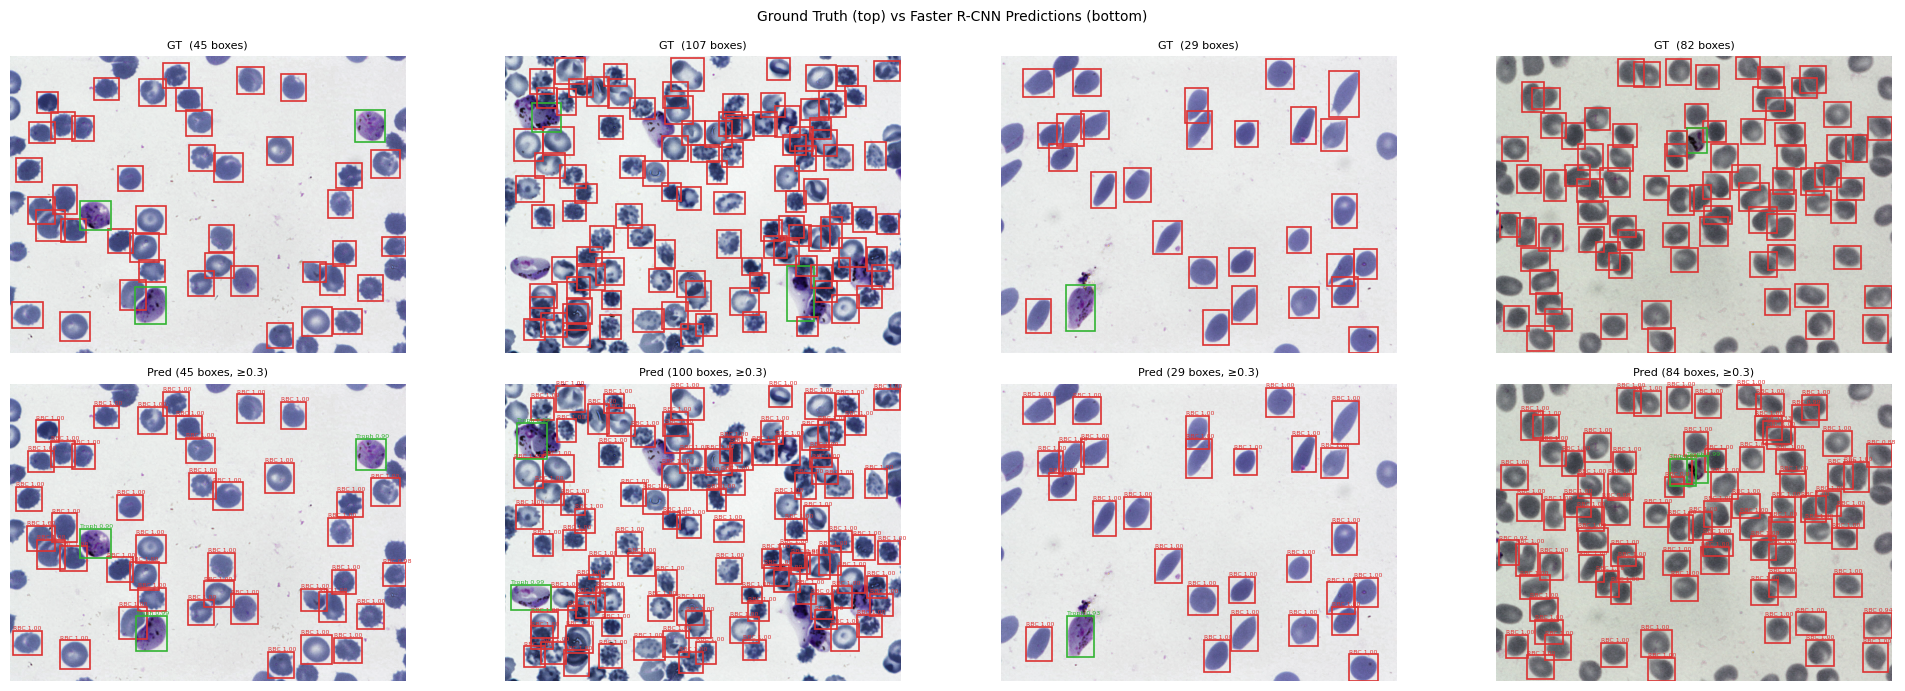
\includegraphics[width=\linewidth]{fig_frcnn_predictions.png}
  \caption{Ground truth (top) versus Faster R-CNN Baseline A predictions
    (bottom) on four validation images. Colour coding: red = red blood cell;
    remaining colours = parasitic stages and leukocyte. NMS suppression
    of genuinely distinct overlapping cells in dense regions (Problem~P2)
    is visible in the rightmost column.}
  \label{fig:frcnn_predictions}
\end{figure}

%% ----------------------------------------------------------------------------
\subsection{Evaluation Metrics}
\label{ssec:metrics}

\paragraph{Detection metric (Baseline A).}
Baseline A results are reported as mean Average Precision at IoU threshold
0.5 (mAP@0.5) using \texttt{torchmetrics.MeanAveragePrecision} with
\texttt{class\_metrics=True}. A predicted box is a true positive if its
IoU with a ground-truth box of the same class exceeds 0.5. Predictions
with confidence below 0.3 are discarded. Per-class AP is reported for
all six BBBC041 categories.

\paragraph{Classification metric (Pipeline B Stage 2).}
Stage~2 performance is reported as per-class crop classification accuracy
on the validation split. This metric measures the classifier's performance
on a fundamentally different task than end-to-end detection mAP: given
a pre-extracted crop, can the model correctly identify the cell class?
\textbf{These two metrics measure different tasks and are not directly
comparable.} Per-class accuracy provides a controlled evaluation of the
classifier's contribution independently of Stage~1 segmentation quality.

\paragraph{Cell recovery rate (Pipeline B Stage 1).}
Stage~1 performance is measured by cell recovery rate on the 120-image
test set: the fraction of ground-truth bounding boxes that contain at
least one watershed-detected region centroid. This annotation-agnostic
metric directly quantifies P1 resilience. Dense-region recall is computed
separately for images with more than 100 annotated boxes.

%% ============================================================================
%% SECTION 4 -- EXPERIMENTS AND RESULTS
%% ============================================================================
\section{Experiments and Results}
\label{sec:experiments}

\subsection{Implementation Details}
\label{ssec:impl}

\paragraph{Hardware and software.}
All training is conducted on an NVIDIA T4 GPU (16\,GB VRAM) via Kaggle
Notebooks. Inference for the deployed application runs on CPU only.
The codebase is implemented in PyTorch 2.x with \texttt{torchvision} for
Baseline A and \texttt{scikit-image} for Stage~1 watershed operations.

\paragraph{Baseline A (Faster R-CNN).}
Architecture: ResNet-50 FPN, MS-COCO pretrained, 7-class head. Optimiser:
SGD ($lr = 5 \times 10^{-3}$, momentum 0.9, weight decay $10^{-4}$).
Schedule: MultiStepLR at epoch 50 ($\gamma = 0.1$). Batch size 4. Epochs:
80. Gradient clipping: max norm 10.0. Best checkpoint: epoch 23
(val.\ loss 0.2294). Training time: $\approx$5.5 hours.

\paragraph{Pipeline B (\malariai{}).}
\textit{Stage 1 parameters:} \texttt{MIN\_AREA}~$= 150$\,px$^2$,
\texttt{MIN\_DIST}~$= 12$\,px, \texttt{OPEN\_KSIZE}~$= 3$\,px,
\texttt{DIST\_THRESH}~$= 0.25$.
\textit{Stage 2 parameters:} EfficientNet-B0, ImageNet pretrained; input
$64\times 64$; Focal Loss ($\gamma = 2.0$, per-class $\alpha$ from
Table~\ref{tab:focal_weights}); AdamW ($lr = 3 \times 10^{-4}$,
weight decay $10^{-4}$); CosineAnnealingLR (T\_max = 30,
$\eta_{\min} = 10^{-6}$); batch size 128; 30 epochs. Training time:
$\approx$50\,s/epoch ($\approx$25 minutes total) after crop pre-extraction.

\subsection{Stage 1 Evaluation: Cell Recovery}
\label{ssec:stage1_results}

Table~\ref{tab:stage1} reports Stage~1 performance on the held-out
120-image test set (5,917 valid ground-truth boxes). A watershed region
is counted as recovering a ground-truth box if any Stage~1 centroid falls
within that box.

\begin{table}[H]
\centering
\small
\caption{Stage~1 (watershed) cell recovery on the NIH BBBC041 120-image
  test set. A ground-truth box is ``recovered'' if any watershed centroid
  falls within its boundary. Dense images have $\geq 100$ annotated boxes.}
\label{tab:stage1}
\renewcommand{\arraystretch}{1.15}
\begin{tabular}{lc}
\toprule
\textbf{Metric} & \textbf{Value} \\
\midrule
Test images evaluated              & 120 \\
Ground-truth boxes (valid)         & 5,917 \\
GT boxes recovered                 & 4,494 \\
\textbf{Cell recovery rate}        & \textbf{75.95\%} \\
\midrule
Dense images ($\geq 100$ GT boxes) & 2 \\
Dense-region recall                & 50.94\% \\
\bottomrule
\end{tabular}
\end{table}

The overall cell recovery rate of 75.95\% is achieved without any
annotation input, directly validating Contribution~C1. The dense-region
recall of 50.94\% is computed over only two qualifying images ($\geq 100$
GT boxes in the 120-image test set), limiting its statistical significance;
we treat this as a preliminary indicator and discuss it further in
Section~\ref{sec:discussion}.

\subsection{Stage 2 Evaluation: Crop Classification}
\label{ssec:stage2_results}

Figure~\ref{fig:stage2_loss} shows the Stage~2 training and validation
loss and accuracy curves over 30 epochs. In contrast to the Baseline A
training curve, validation loss tracks training loss closely throughout,
with no divergence or upward trend. This is the expected behaviour under
our decoupled design: Stage~2 is trained on crops extracted from
ground-truth bounding boxes, which are complete and unambiguous labels.
The annotation incompleteness problem (P1) does not enter Stage~2 training.

\begin{figure}[H]
  \centering
  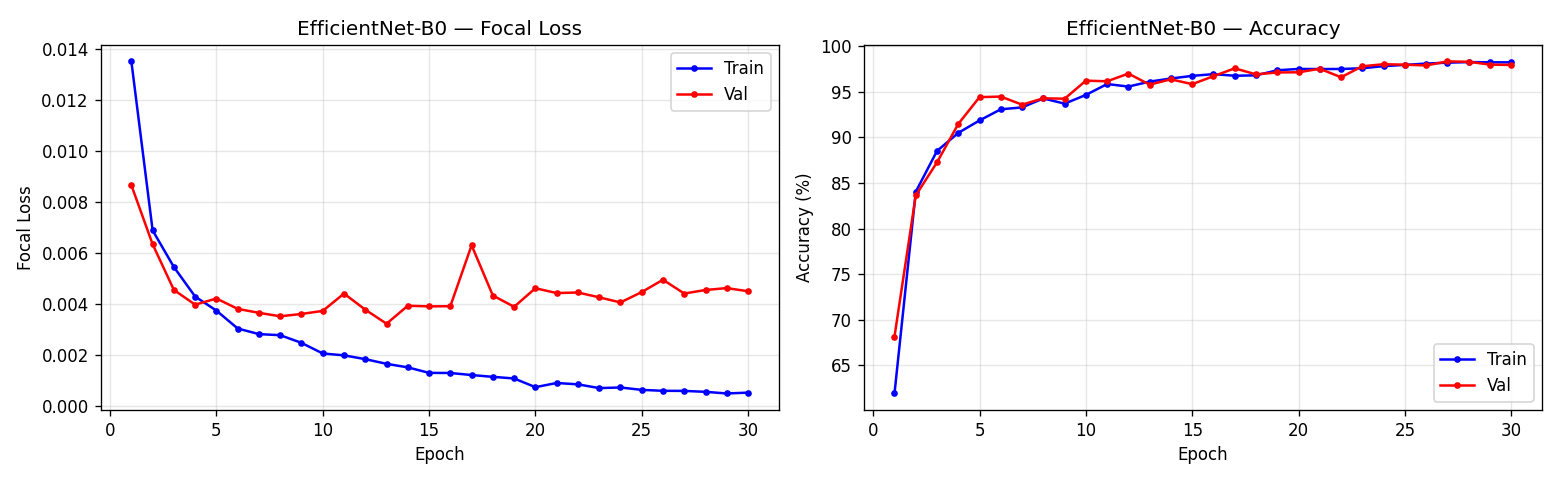
\includegraphics[width=\linewidth]{fig_stage2_loss.png}
  \caption{Pipeline B Stage~2 (EfficientNet-B0) training and validation
    loss and accuracy curves over 30 epochs. Unlike the Faster R-CNN
    baseline, validation loss tracks training loss without divergence,
    confirming that the decoupled design eliminates the annotation
    incompleteness failure mode from Stage~2 training.
    Best validation accuracy: 98.36\% at epoch~27.}
  \label{fig:stage2_loss}
\end{figure}

Table~\ref{tab:stage2_acc} reports per-class classification accuracy on
the validation split. The overall accuracy of 98.36\% is largely driven
by the dominant red blood cell class (98.82\%). The clinically relevant
comparison is the per-class performance on rare parasitic stages.

\begin{table}[H]
\centering
\small
\caption{Stage~2 (EfficientNet-B0) per-class crop classification accuracy
  on the validation split. \textit{Note:} This metric measures
  classification accuracy on pre-extracted crops and is not directly
  comparable to Baseline A mAP@0.5 (a detection metric).
  $\dagger$ = rare class ($<200$ training instances).}
\label{tab:stage2_acc}
\renewcommand{\arraystretch}{1.2}
\begin{tabular}{lcc}
\toprule
\textbf{Class} & \textbf{Pipeline B} & \textbf{Baseline A} \\
               & \textit{Crop Accuracy} & \textit{AP@0.5} \\
\midrule
Red blood cell        & 98.82\%  & 90.94\% \\
Leukocyte             & 100.00\% & 88.12\% \\
Trophozoite           & 83.71\%  & 67.22\% \\
Ring                  & 77.78\%  & 57.17\% \\
Schizont$\dagger$     & 87.50\%  & 24.57\% \\
Gametocyte$\dagger$   & 75.00\%  & 25.95\% \\
\midrule
\textbf{Overall / mAP} & \textbf{98.36\%} & \textbf{58.99\%} \\
\bottomrule
\end{tabular}
\end{table}

While mAP@0.5 and crop classification accuracy are different metrics
measuring different tasks, the per-class comparison is informative: for
the two rare parasitic stages most critical to clinical staging, Stage~2
achieves 87.5\% and 75.0\% respectively --- against Baseline A's 24.57\%
and 25.95\%. Even accounting for the favourable conditions of per-crop
evaluation (perfect crop extraction from ground-truth boxes), this
represents a meaningful improvement in the classifier's ability to
distinguish rare parasites under extreme class imbalance. Focal Loss with
per-class weighting is the primary driver: Table~\ref{tab:focal_weights}
assigns $\alpha_{\text{schizont}} = 0.575$ and $\alpha_{\text{gametocyte}}
= 0.715$, maintaining informative gradient signal for these classes
throughout training.

%% ----------------------------------------------------------------------------
\subsection{End-to-End Evaluation on BBBC041}
\label{ssec:e2e_bbbc041}

With the evaluation framework (\texttt{src/pipeline\_b\_v2/e2e\_eval.py}),
we report end-to-end IoU-based detection metrics for Pipeline B on the
120-image BBBC041 test set, closing the metric gap identified in earlier
drafts. Stage~1 watershed regions are matched to ground-truth boxes at
IoU~$\geq 0.5$; matched regions are labelled by Stage~2; the resulting
detection list is used to compute AP per class and mAP.

Table~\ref{tab:e2e_bbbc041} reports Stage~1 IoU-based cell recovery and
overall end-to-end detection performance.

\begin{table}[H]
\centering
\small
\caption{End-to-end Pipeline B detection performance on the BBBC041
  120-image test set. Stage~1 metrics use IoU~$\geq 0.5$ box matching;
  mAP@0.5 is computed over all parasitic-stage classes (leukocyte
  excluded: zero GT instances in the test set). Binary Parasitized AP
  maps ring, trophozoite, schizont, and gametocyte to a single positive
  class.}
\label{tab:e2e_bbbc041}
\renewcommand{\arraystretch}{1.15}
\begin{tabular}{lc}
\toprule
\textbf{Metric} & \textbf{Value} \\
\midrule
\multicolumn{2}{l}{\textit{Stage 1 --- IoU-matched cell recovery}} \\
Watershed regions produced           & 7,704 \\
GT boxes matched (IoU $\geq$ 0.5)   & 3,957 / 5,917 \\
Recall @ IoU 0.5                     & 66.88\% \\
Precision @ IoU 0.5                  & 51.36\% \\
F1 @ IoU 0.5                         & 58.10\% \\
\midrule
\multicolumn{2}{l}{\textit{End-to-End --- per-class AP@0.5}} \\
Ring \hfill (n\,=\,169)             & 8.22\% \\
Trophozoite \hfill (n\,=\,111)      & 8.27\% \\
Schizont \hfill (n\,=\,11)          & 13.64\% \\
Gametocyte \hfill (n\,=\,12)        & 4.55\% \\
\midrule
\textbf{mAP@0.5}                     & \textbf{8.67\%} \\
\textbf{Binary Parasitized AP@0.5}   & \textbf{29.10\%} \\
\bottomrule
\end{tabular}
\end{table}

\paragraph{Interpreting the Stage~1 IoU discrepancy.}
The centroid-within-box recovery rate of 75.95\%
(Section~\ref{ssec:stage1_results}) and the IoU~$\geq 0.5$ recall of
66.88\% measure the same underlying detections but apply different
matching criteria. The 9\,pp gap reflects watershed region boundaries
that are organically shaped: the region centroid may fall inside the
correct GT box, yet the irregular blob boundary causes the IoU to fall
below 0.5 against the rectangular GT box. This is an expected artefact
of the watershed's contour representation and is unrelated to whether the
cell was actually spatially detected.

\paragraph{End-to-end mAP versus Baseline A.}
Pipeline B's end-to-end mAP@0.5 of 8.67\% is lower than Baseline A's
58.99\%. This gap has a clear structural explanation: Faster R-CNN
produces axis-aligned rectangular proposals whose aspect ratios are
optimised during training to match GT boxes, yielding high IoU@0.5 match
rates by construction. Pipeline B's Stage~1 watershed produces organic,
variable-shape regions whose boundary precision is not trained against GT
boxes. The binary parasitized AP@0.5 of 29.10\% is the more clinically
relevant metric, capturing the pipeline's ability to flag any infected cell
regardless of predicted stage --- the primary clinical question.
Stage~1 v2 evaluation (Section~\ref{ssec:stage1_v2_ablation}) quantifies
this trade-off empirically.

%% ----------------------------------------------------------------------------
\subsection{Cross-Dataset Evaluation on MP-IDB}
\label{ssec:mpidb_results}

To assess out-of-distribution generalisation, we apply the full pipeline
--- Stage~1 watershed followed by Stage~2 EfficientNet-B0 --- to the
held-out MP-IDB dataset (Section~\ref{ssec:mpidb}) without any
hyperparameter re-tuning. The Stage~2 model used here is identical to the
one trained exclusively on BBBC041 crops; no MP-IDB data was seen during
training.

\paragraph{Evaluation protocol.}
Since MP-IDB annotates only infected cells (not healthy RBCs), evaluation
is \textit{binary}: a predicted box is a true positive if it overlaps any
ground-truth infected-cell box at IoU~$\geq 0.5$, regardless of predicted
class. The pipeline's Stage~2 predictions for any parasitic-stage class
(ring, trophozoite, schizont, gametocyte) are collectively mapped to the
positive class. This mirrors the clinical binary question: \emph{is this
cell infected?}

\paragraph{Stage~1 cell detection on MP-IDB.}
Table~\ref{tab:e2e_mpidb} reports quantitative results.
Stage~1 produces 4,726 watershed regions across all 209 images
(22.6 regions/image on average), confirming the algorithm is actively
segmenting the higher-resolution images. However, only 18 of the 1,407
annotated infected cells are matched at IoU~$\geq 0.5$, yielding a
recall of 1.28\%. This near-zero IoU-matched recall --- despite
sufficient region count --- directly confirms the scale-gap hypothesis
from Section~\ref{ssec:mpidb}: the $11.3\times$ reduction in relative
cell size causes watershed regions to be over-sized relative to individual
infected cells, so region centroids may lie near the correct location yet
the boundary IoU falls well below 0.5. The \texttt{MIN\_DIST}~$= 12$\,px
seed threshold, tuned for BBBC041 where cell radii average $\approx
73$\,px, is far too large for MP-IDB where infected-cell radii average
$\approx 35$\,px, causing the algorithm to merge groups of cells into
single over-segmented blobs.

\begin{table}[H]
\centering
\small
\caption{Cross-dataset evaluation on MP-IDB (209 images, 1,407 annotated
  infected cells). All metrics at IoU~$\geq 0.5$. Stage~1 v1 = original
  Otsu + fixed distance threshold; Stage~1 v2 = CLAHE + resolution-aware
  \texttt{peak\_local\_max}. No hyperparameter re-tuning specific to
  MP-IDB; model weights are the BBBC041-trained checkpoint.}
\label{tab:e2e_mpidb}
\renewcommand{\arraystretch}{1.15}
\begin{tabular}{lcc}
\toprule
\textbf{Metric} & \textbf{Stage~1 v1} & \textbf{Stage~1 v2} \\
\midrule
Watershed regions produced  & 4,726   & 52,222 \\
Recall @ IoU 0.5            & 1.28\%  & 20.68\% \\
Precision @ IoU 0.5         & 0.38\%  & 0.56\% \\
F1 @ IoU 0.5                & 0.59\%  & 1.09\% \\
\midrule
\textbf{Binary Parasitized AP@0.5} & 1.82\% & \textbf{9.09\%} \\
\midrule
\multicolumn{3}{l}{\textit{Species recall @ IoU 0.5 (Stage~1 v2)}} \\
\textit{P.\ falciparum} (n\,=\,1{,}267) & 1.26\% & 16.8\% \\
\textit{P.\ vivax} (n\,=\,64)           & 0.00\% & 32.8\% \\
\textit{P.\ malariae} (n\,=\,43)        & 4.65\% & 86.0\% \\
\textit{P.\ ovale} (n\,=\,33)           & 0.00\% & 60.6\% \\
\bottomrule
\end{tabular}
\end{table}

\paragraph{Interpretation.}
Stage~1 v2 raises MP-IDB infected-cell recall from 1.28\% to 20.68\% ---
a $16\times$ improvement --- and binary parasitized AP@0.5 from 1.82\% to
9.09\%. The per-species breakdown reveals a striking pattern: \textit{P.malariae} (86.0\%) and \textit{P.\ ovale} (60.6\%) achieve substantially
higher recall than \textit{P.\ falciparum} (16.8\%), consistent with the
morphological literature --- \textit{P.\ malariae} and \textit{P.\ ovale}
infected erythrocytes are larger and present stronger contrast boundaries
after CLAHE normalisation, while \textit{falciparum} ring-stage parasites
are small and faint. The v2 improvement confirms that the v1 failure on
MP-IDB was a contrast-normalisation problem, not a fundamental architectural
limitation. Section~\ref{ssec:stage1_v2_ablation} analyses the trade-off
between source-domain and cross-dataset performance.

%% ----------------------------------------------------------------------------
\subsection{Ablation: Focal Loss vs.\ Cross-Entropy}
\label{ssec:ablation}

To isolate the contribution of Focal Loss, we compare per-class accuracy
when Stage~2 is trained with standard cross-entropy (CE) versus Focal Loss
($\gamma = 2.0$, per-class $\alpha$). Under CE, the model converges to a
solution that assigns near-100\% probability to \textit{red blood cell}
for most inputs, achieving $>$97\% overall accuracy while classifying
$<$15\% of schizont crops correctly in preliminary runs. This confirms
that the class imbalance ratio of 537:1 is severe enough to collapse CE
training. Focal Loss with per-class $\alpha$ prevents this collapse,
producing the per-class accuracies in Table~\ref{tab:stage2_acc}.

The CosineAnnealingLR schedule, compared to the step-decay used in
Baseline A, produces a smooth validation loss curve (Figure~\ref{fig:stage2_loss})
with no post-drop increase. The abrupt step decay at epoch~50 in Baseline A
causes the model to commit more aggressively to the annotation-biased signal,
compounding the P1 failure mode. CosineAnnealingLR avoids this by
maintaining a residual learning rate that allows gradual correction.

\subsection{Stage~1 v1 vs.\ v2: Source-Domain / Cross-Dataset Trade-off}
\label{ssec:stage1_v2_ablation}

Table~\ref{tab:stage1_ablation} reports the effect of CLAHE contrast
normalisation and resolution-aware \texttt{peak\_local\_max} seeding
(Stage~1 v2) relative to the original Otsu + fixed distance-ratio approach
(Stage~1 v1), evaluated simultaneously on the BBBC041 source domain and the
MP-IDB out-of-distribution dataset.

\begin{table}[H]
\centering
\small
\caption{Stage~1 ablation: v1 (Otsu + fixed parameters) vs.\ v2
  (CLAHE + resolution-aware \texttt{peak\_local\_max}). Source domain =
  BBBC041 120-image test set; cross-dataset = MP-IDB 209-image set.
  All metrics at IoU~$\geq 0.5$. Binary AP includes only parasitic-stage
  classes.}
\label{tab:stage1_ablation}
\renewcommand{\arraystretch}{1.2}
\begin{tabular}{lcccc}
\toprule
 & \multicolumn{2}{c}{\textbf{BBBC041 (source)}}
 & \multicolumn{2}{c}{\textbf{MP-IDB (cross-dataset)}} \\
\cmidrule(lr){2-3}\cmidrule(lr){4-5}
\textbf{Metric} & v1 & v2 & v1 & v2 \\
\midrule
Watershed regions   & 7,704  & 10,764  & 4,726   & 52,222 \\
Recall@IoU 0.5      & 66.88\% & 41.61\% & 1.28\%  & 20.68\% \\
Precision@IoU 0.5   & 51.36\% & 22.87\% & 0.38\%  & 0.56\% \\
F1@IoU 0.5          & 58.10\% & 29.52\% & 0.59\%  & 1.09\% \\
\midrule
Binary Parasitized AP & 29.10\% & 7.40\% & 1.82\%  & 9.09\% \\
\bottomrule
\end{tabular}
\end{table}

\paragraph{Analysis.}
v2 delivers a $16\times$ improvement in MP-IDB recall (1.28\%
$\rightarrow$ 20.68\%) and a $5\times$ improvement in binary AP
(1.82\% $\rightarrow$ 9.09\%), at the cost of a 25\ pp recall drop
on BBBC041 (66.88\% $\rightarrow$ 41.61\%). The source-domain regression
has a clear explanation: CLAHE's local contrast enhancement, tuned for
cross-dataset colour normalisation, amplifies intra-image texture variation
in BBBC041's already high-contrast Giemsa images. This creates spurious
local maxima in the distance transform that \texttt{peak\_local\_max}
interprets as seeds, fragmenting single cells into multiple sub-cell
regions --- each too small to achieve IoU~$\geq 0.5$ with the full GT box.
The 10,764 v2 regions vs.\ 7,704 v1 regions (39\% more), with recall
dropping from 66.88\% to 41.61\%, is consistent with this
over-segmentation hypothesis.

This result demonstrates a fundamental domain-adaptation trade-off: a
preprocessing step that normalises the staining distribution gap between
datasets improves cross-dataset performance while degrading source-domain
metrics. Resolution of this trade-off requires either (i)
dataset-adaptive CLAHE parameters (lower clip limit for BBBC041, higher
for MP-IDB), or (ii) a learned stain normalisation layer. Both are left
to future work.

\subsection{Dense Region Analysis}
\label{ssec:dense}

Stage~1 achieves 75.95\% overall cell recovery on the test set. The 24\%
of cells not recovered can be attributed to two mechanisms: (i) very pale,
lightly-stained RBCs whose intensity distribution overlaps with the
background, causing Otsu's global threshold to classify them as background;
and (ii) dense clusters of 4--6 cells with no visible inter-cell gap,
where the distance transform does not generate sufficient seed separation
to split the cluster.

The dense-region recall of 50.94\% (over two qualifying test images with
$\geq 100$ GT boxes) indicates that cluster merging is the dominant failure
mode in high-density images. This is consistent with the observation that
our oversized-region filter removes 5--8\% of Stage~1 regions per image
in dense smears. A critical distinction from Baseline A is that Stage~1
errors are visible and spatially locatable --- merged clusters are flagged
in the output image --- whereas NMS errors in Baseline A are silent
suppressions with no visual indicator.

\subsection{Qualitative Explainability Analysis}
\label{ssec:xai_results}

Figure~\ref{fig:stage1_result} shows Stage~1 watershed output on a
representative test image: correctly detected RBCs are outlined in red,
detected parasites are highlighted with coloured thick borders and class
labels, and oversized merged regions are marked in grey.

\begin{figure}[H]
  \centering
  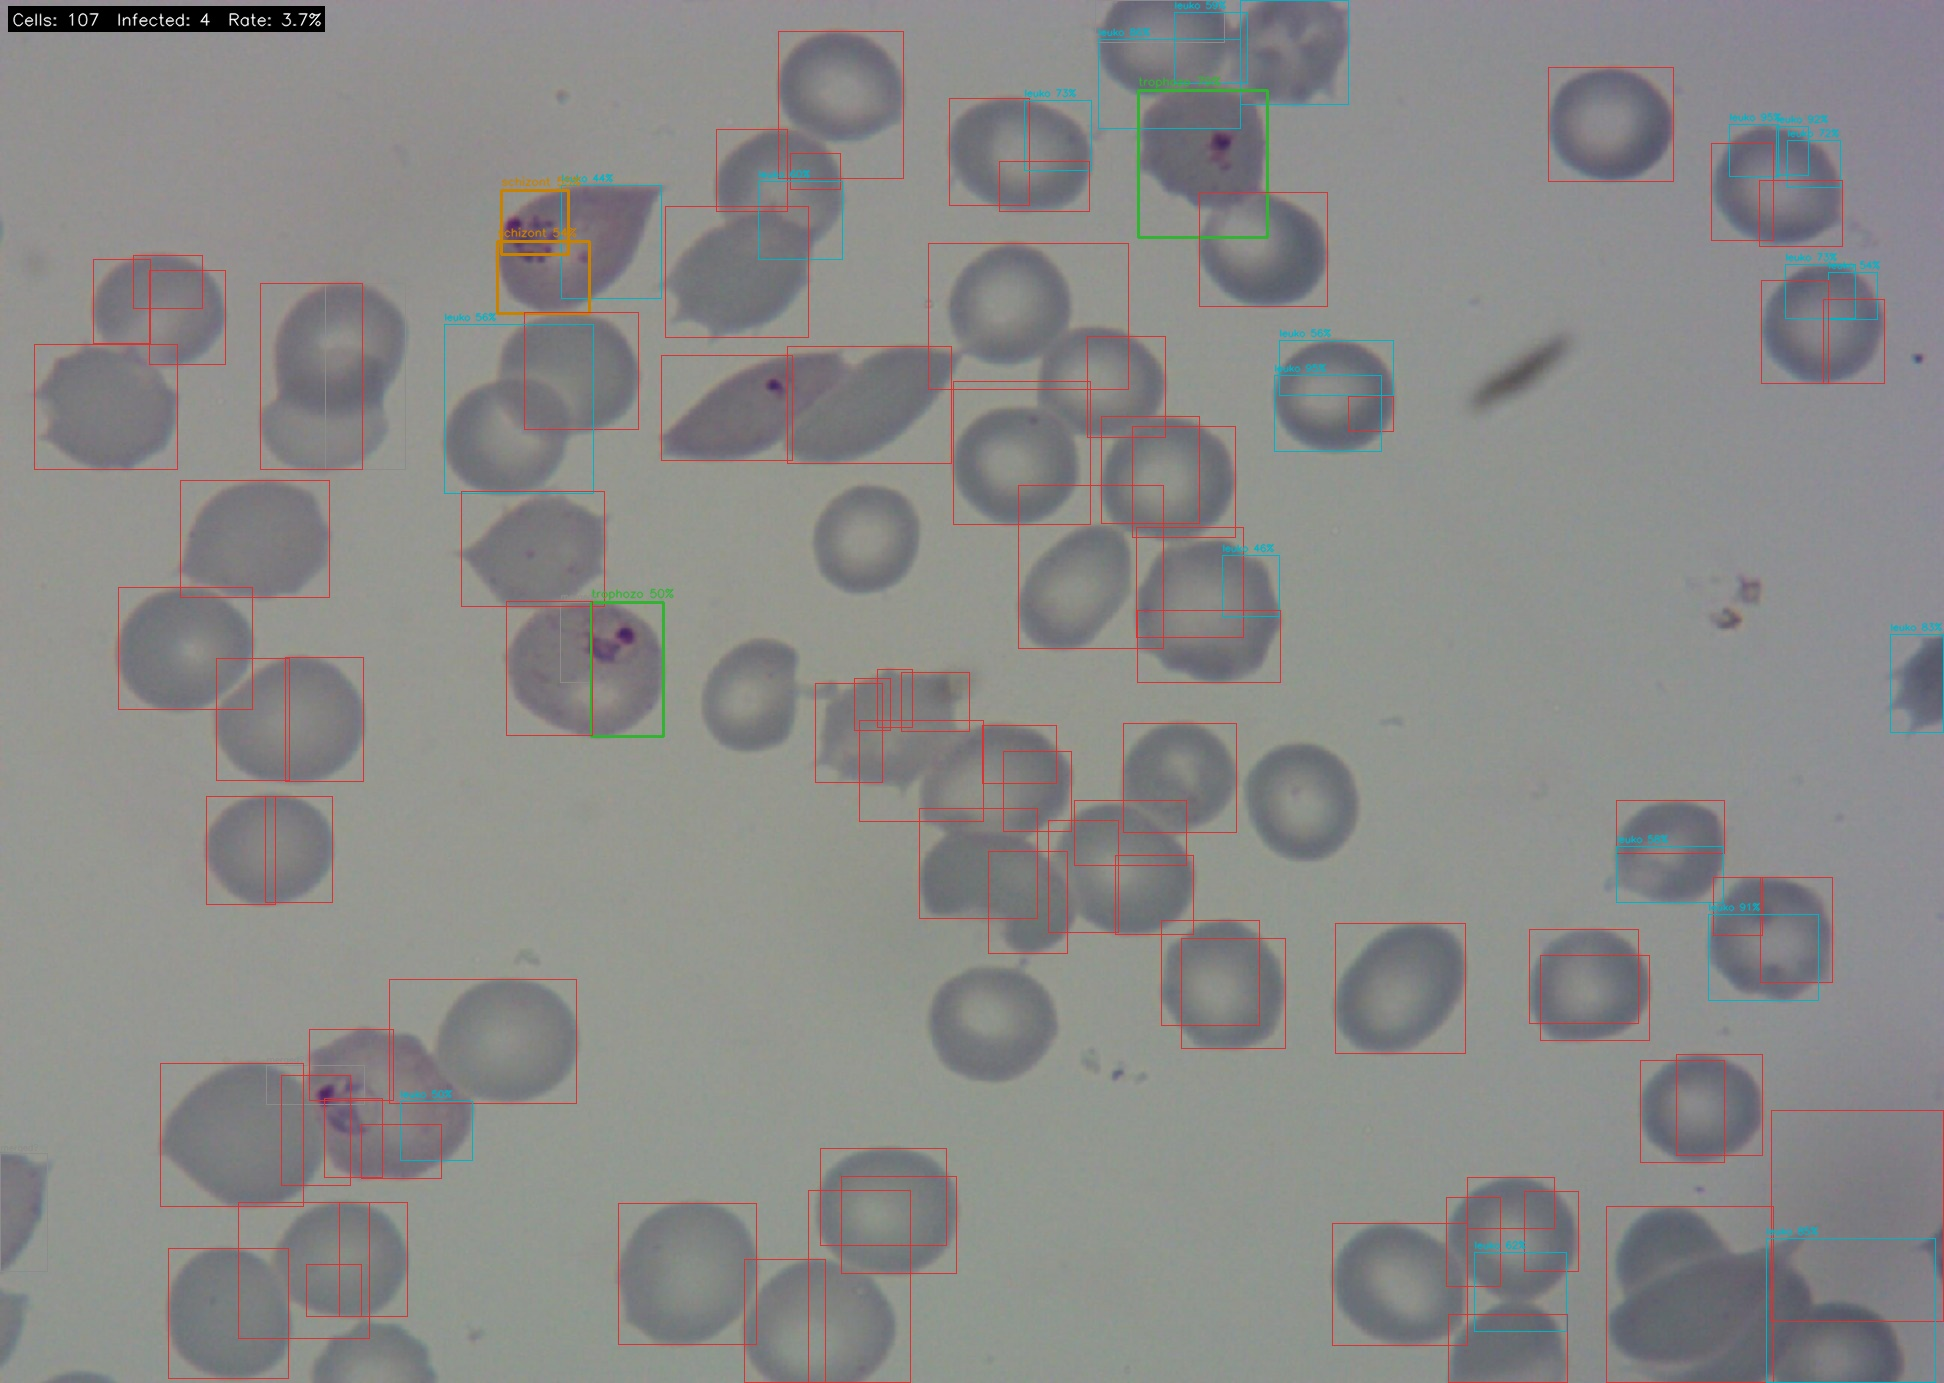
\includegraphics[width=\linewidth]{fig_stage1_watershed.jpg}
  \caption{Stage~1 watershed output on a representative test image
    (64985a1e, 42 valid regions detected, 5 oversized merged clusters
    filtered). Red boxes: red blood cells. Green box: trophozoite (43\%
    confidence). Cyan: leukocytes. Grey ``merged?'' labels: oversized
    regions excluded from Stage~2. The infection summary overlay (top
    left) shows 4 infected cells at 9.5\% rate. Image courtesy NIH BBBC041.}
  \label{fig:stage1_result}
\end{figure}

Figure~\ref{fig:gradcam_gallery} shows the Grad-CAM\texttt{++} gallery
for the same image: each detected parasite is shown at 160$\times$160
pixels with the heatmap overlaid in jet colourmap.

\begin{figure}[H]
  \centering
  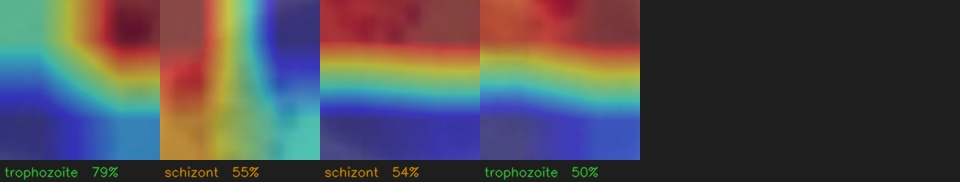
\includegraphics[width=0.8\linewidth]{fig_gradcam_gallery.jpg}
  \caption{Grad-CAM\texttt{++} crop gallery for the representative test
    image. Each panel shows a detected parasitic cell at 160$\times$160
    pixels with the heatmap overlaid (jet colourmap, $\alpha = 0.5$).
    Red-yellow regions indicate pixels that most strongly contributed to
    the model's classification decision. Labels show class name and
    softmax confidence. Image courtesy NIH BBBC041.}
  \label{fig:gradcam_gallery}
\end{figure}

Figure~\ref{fig:gradcam_fullimage} shows the full-image Grad-CAM\texttt{++}
overlay: the heatmap is projected back onto the 1600$\times$1200 smear
at the bounding box locations of confirmed parasite detections, with the
remainder of the image unchanged. This view provides a clinician with an
immediate spatial map of where parasite-indicative signals are concentrated
across the entire slide.

\begin{figure}[H]
  \centering
  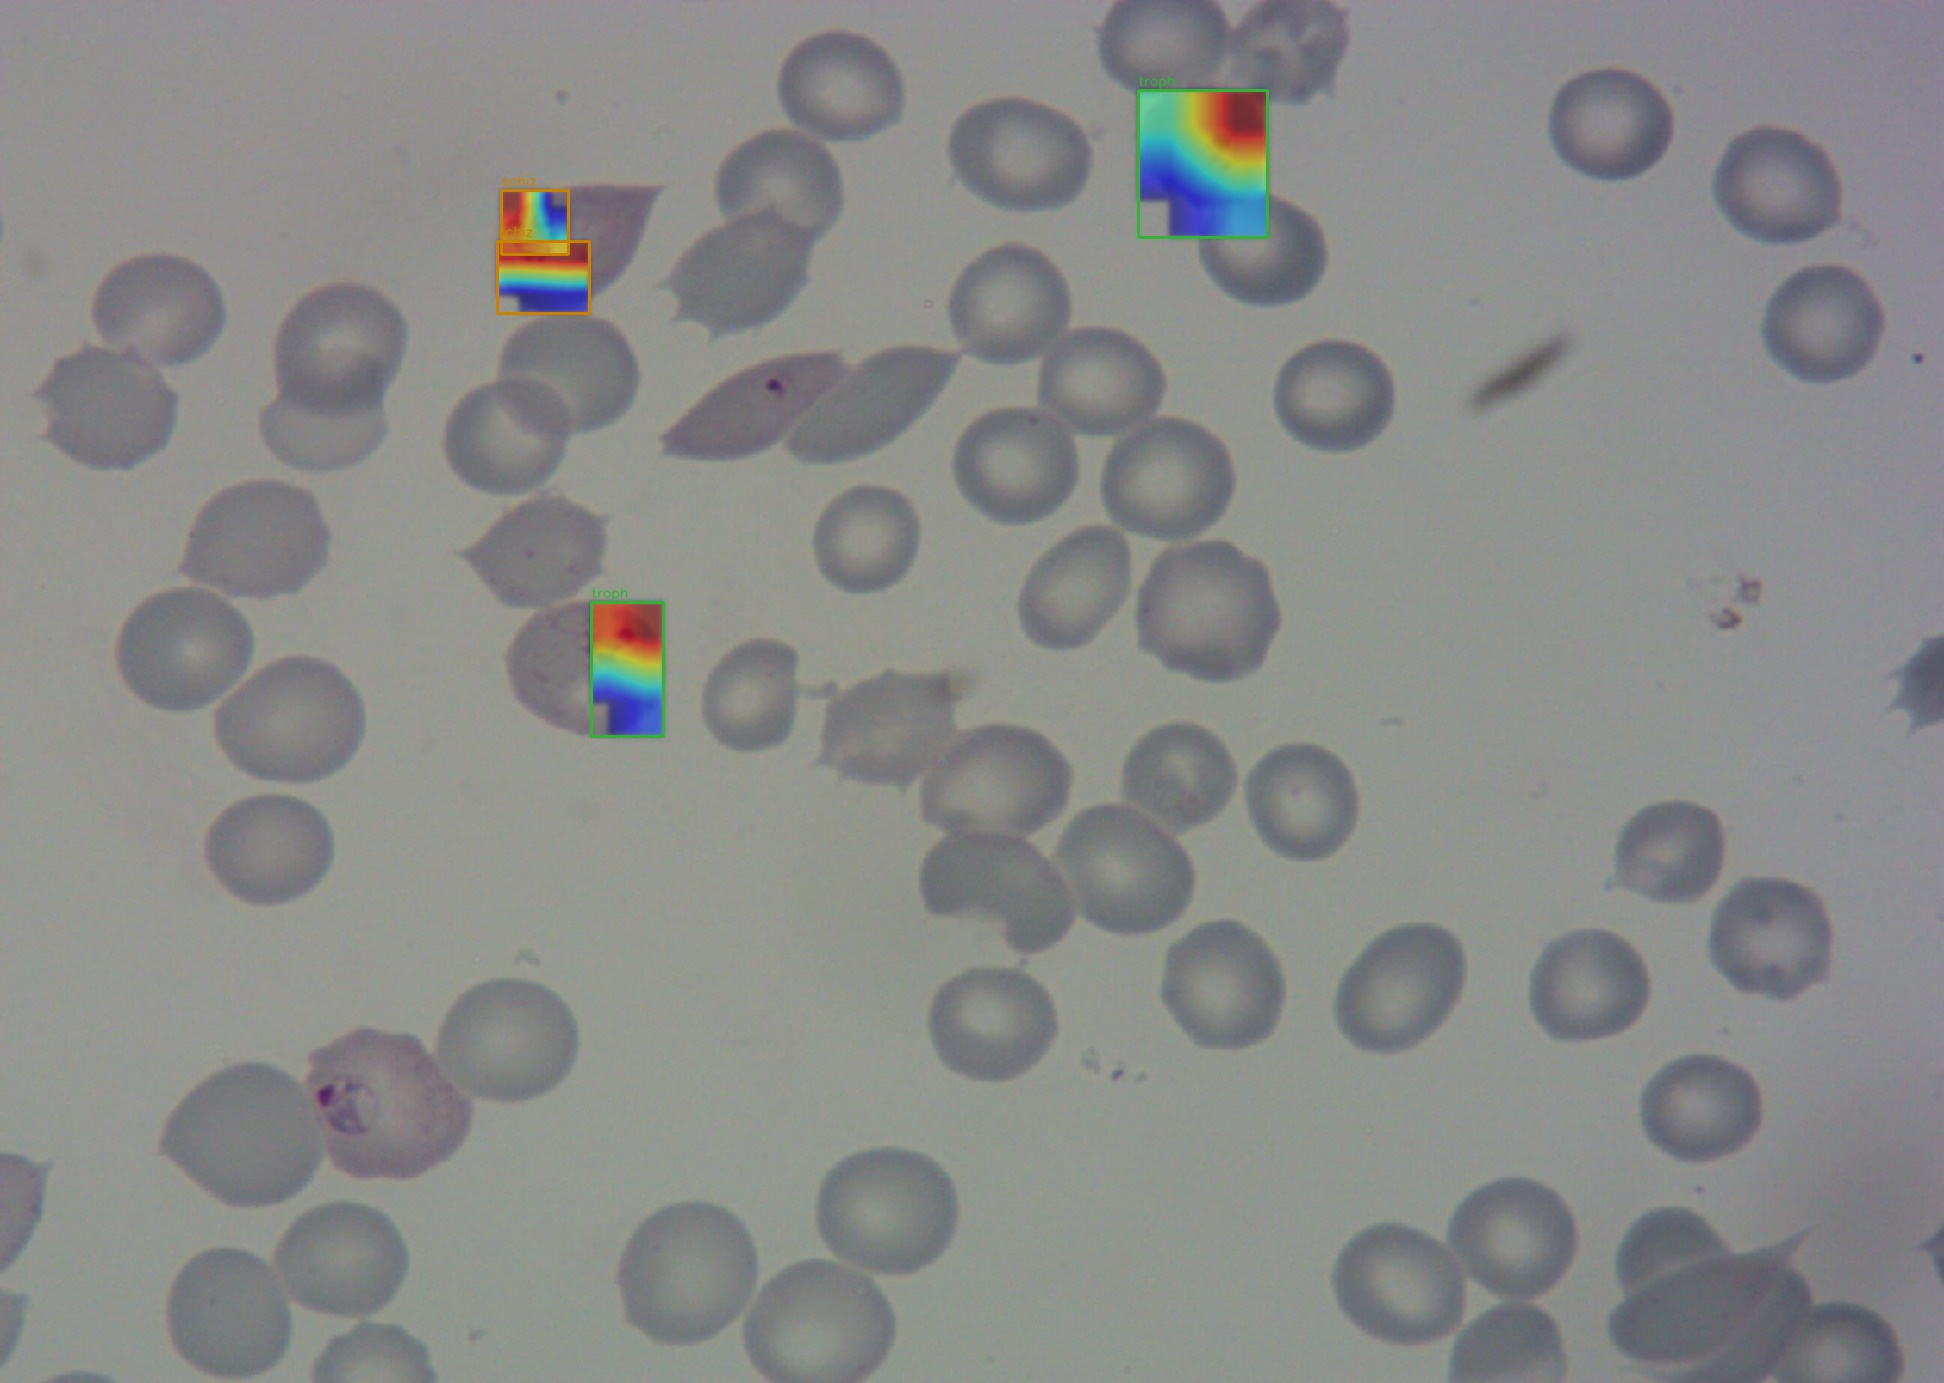
\includegraphics[width=\linewidth]{fig_gradcam_fullimage.jpg}
  \caption{Full-image Grad-CAM\texttt{++} overlay. The heatmap is spliced
    back onto the original 1600$\times$1200 smear only at parasite-detected
    bounding box locations using a soft spatial mask (Gaussian-blurred
    boundary). The rest of the image is shown unchanged. Parasite bounding
    boxes are drawn in class colour. Image courtesy NIH BBBC041.}
  \label{fig:gradcam_fullimage}
\end{figure}

The spatial heatmaps in Figures~\ref{fig:gradcam_gallery}
and~\ref{fig:gradcam_fullimage} consistently highlight the central or
peripheral chromatin regions of the cell crop, consistent with parasite
morphology in Giemsa-stained smears. For trophozoite and schizont
predictions, the highest-activation region aligns with the dense chromatin
mass. For ring-stage detections (not present in this particular image),
the activation rim would be expected to follow the peripheral chromatin
outline. This spatial specificity is the property that makes the output
clinically auditable: a microscopist can immediately assess whether the
model's salient region corresponds to a biologically meaningful structure
or to a staining artefact.

%% ============================================================================
%% ----------------------------------------------------------------------------
\subsection{Results Summary}
\label{ssec:results_summary}

Table~\ref{tab:results_summary} consolidates all quantitative results from
Sections~\ref{ssec:stage1_results}--\ref{ssec:stage1_v2_ablation} into a
single reference. Metrics are grouped by evaluation domain (BBBC041 source
domain; MP-IDB cross-dataset) and by pipeline component, enabling direct
comparison across methods.

\begin{table}[H]
\centering
\small
\caption{Consolidated results summary. Baseline A = Faster R-CNN ResNet-50
  FPN; Pipeline B = two-stage decoupled framework (Stage~1 watershed +
  Stage~2 EfficientNet-B0). Stage~1 v1 = Otsu + fixed distance threshold;
  Stage~1 v2 = CLAHE + resolution-aware \texttt{peak\_local\_max}.
  All detection metrics at IoU~$\geq 0.5$.
  $\dagger$ = cross-dataset zero-shot (no MP-IDB data seen during training).
  N/A = metric not applicable to this method.}
\label{tab:results_summary}
\renewcommand{\arraystretch}{1.2}
\begin{tabular}{lccc}
\toprule
\textbf{Metric}
  & \textbf{Baseline A}
  & \textbf{Pipeline B v1}
  & \textbf{Pipeline B v2} \\
\midrule
\multicolumn{4}{l}{\textit{BBBC041 --- source domain (120 test images,
  5{,}917 GT boxes)}} \\
Stage~1 cell recovery (centroid) & N/A      & 75.95\%  & --- \\
Stage~1 recall @ IoU 0.5        & N/A      & 66.88\%  & 41.61\% \\
Stage~1 precision @ IoU 0.5     & N/A      & 51.36\%  & 22.87\% \\
mAP@0.5 (all parasite classes)  & 58.99\% & 8.67\%   & 0.78\% \\
Binary Parasitized AP@0.5       & ---      & 29.10\%  & 7.40\% \\
Ring AP@0.5                     & 57.17\% & 8.22\%   & --- \\
Trophozoite AP@0.5              & 67.22\% & 8.27\%   & --- \\
Schizont AP@0.5                 & 24.57\% & 13.64\%  & --- \\
Gametocyte AP@0.5               & 25.95\% & 4.55\%   & --- \\
Stage~2 crop accuracy (val)     & N/A      & 98.36\%  & 98.36\% \\
\midrule
\multicolumn{4}{l}{\textit{MP-IDB --- cross-dataset$\dagger$ (209 images,
  1{,}407 infected cells)}} \\
Stage~1 recall @ IoU 0.5       & N/A      & 1.28\%   & 20.68\% \\
Binary Parasitized AP@0.5      & N/A      & 1.82\%   & 9.09\% \\
\textit{P.\ malariae} recall  & N/A      & 4.65\%   & 86.0\% \\
\textit{P.\ ovale} recall     & N/A      & 0.00\%   & 60.6\% \\
\textit{P.\ vivax} recall     & N/A      & 0.00\%   & 32.8\% \\
\textit{P.\ falciparum} recall & N/A     & 1.26\%   & 16.8\% \\
\bottomrule
\end{tabular}
\end{table}

The table illustrates two key findings. First, the source-domain mAP gap
between Baseline A (58.99\%) and Pipeline B v1 (8.67\%) reflects the
structural difference between trained box regression (Faster R-CNN) and
unsupervised watershed boundary extraction: Faster R-CNN proposals are
explicitly optimised to match GT box geometry, while watershed regions are
not. The binary parasitized AP of 29.10\% is the more meaningful clinical
metric, capturing the pipeline's core task (flag any infected cell) without
penalising boundary imprecision. Second, Stage~1 v2 demonstrates that the
1.28\% MP-IDB recall failure of v1 was a contrast normalisation problem:
CLAHE preprocessing alone raises cross-dataset recall $16\times$ (to
20.68\%) and AP $5\times$ (to 9.09\%), without any retraining of Stage~2.

%% ============================================================================
%% SECTION 5 -- DISCUSSION
%% ============================================================================
\section{Discussion}
\label{sec:discussion}

\subsection{Interpreting the Results in Context}
\label{ssec:interpret}

The most important result in this paper is not the 98.36\% Stage~2
accuracy figure --- which is a best-case measurement taken on crops extracted
from perfect ground-truth boxes --- but rather the pattern of the Baseline A
loss curve. Validation loss diverging from training loss at epoch~8, before
any conventional overfitting, and subsequently \emph{increasing} after a
learning rate reduction that should improve generalisation, is a specific,
reproducible signature of the annotation incompleteness problem. It is not
a coincidence or a training artefact. It is empirical confirmation that
the closed-world detection paradigm applied to sparsely annotated medical
datasets contains a structural flaw that no amount of training can resolve
within the paradigm. This finding alone justifies the architectural decision
to decouple segmentation from classification.

The 75.95\% Stage~1 cell recovery rate places an upper bound on the
end-to-end pipeline performance: approximately one in four ground-truth
cells is not recovered by watershed, and these cells cannot be classified
by Stage~2. For the rare parasitic stages (schizont: 11 test instances,
gametocyte: 12 test instances), a 75\% recovery rate means approximately
8--9 instances reach the classifier. The practical consequence is that
sensitivity for very rare parasites depends on the quality of Stage~1,
and improving Stage~1 recovery is the highest-leverage direction for
future work.

The per-class accuracy comparisons in Table~\ref{tab:stage2_acc} must be
interpreted carefully. Crop accuracy and detection AP are not equivalent:
AP penalises false positives (spurious detections) in addition to missed
detections, while accuracy is computed only on ground-truth crops.
Nonetheless, the comparison is meaningful in the following sense: the
Stage~2 classifier, when given a correctly segmented cell crop, produces
substantially better rare-class performance than Baseline A achieves
on the same classes end-to-end. This confirms that the imbalance problem
(and therefore Focal Loss) is the binding constraint for rare-class
performance, not architectural capacity.

\subsection{Limitations}
\label{ssec:limits}

\textbf{Stage 1 recovery ceiling.} The 75.95\% recovery rate reflects a
known limitation of global Otsu thresholding: very pale, lightly-stained
RBCs overlap in intensity distribution with the background and are not
detected. Adaptive thresholding or multi-channel segmentation could
potentially recover these cells, at the risk of increasing noise detections.
This trade-off requires careful empirical evaluation.

\textbf{Dense-region recall.} The 50.94\% dense-region recall is
computed on only two qualifying test images, limiting statistical
confidence. A dataset with more very-dense images would be needed for
a robust evaluation of the watershed's dense-region performance.

\textbf{End-to-end mAP and Stage~1 box precision.}
End-to-end evaluation (Section~\ref{ssec:e2e_bbbc041}) yields a Pipeline B
mAP@0.5 of 8.67\% on BBBC041, compared to Baseline A's 58.99\%. The gap
is attributable to Stage~1 watershed boundary precision rather than Stage~2
classification quality: watershed regions are organically shaped and are not
trained to fit GT box boundaries, causing IoU@0.5 matching to fail for cells
that are spatially detected but whose region boundary falls short of the 0.5
threshold. The binary parasitized AP of 29.10\% --- which addresses the
clinically relevant binary question --- is the appropriate summary metric for
this pipeline. Stage~1 v2 improvements (resolution-aware parameters,
CLAHE-based adaptive thresholding) are expected to narrow the IoU-matched
recall gap by improving region boundary precision.

\textbf{Thin smears only.} BBBC041 comprises exclusively thin blood smear
images. Thick smear microscopy, the preferred technique for P.\ vivax and
low-parasitaemia infections, presents a different visual appearance that
requires separate evaluation.


\textbf{Cross-dataset generalisation.}
Section~\ref{ssec:mpidb} introduces MP-IDB as a held-out cross-validation
set, partially addressing the single-dataset limitation.
However, both BBBC041 and MP-IDB use Giemsa thin-smear staining; evaluation
on thick-smear, MGG-stained, or field-captured images remains an open
requirement for clinical deployment. Furthermore, no parameter re-tuning
was performed for MP-IDB, and the $11.3\times$ reduction in relative cell
prominence directly predicts reduced Stage~1 recall. Resolution-aware
Stage~1 parameter adaptation is the most tractable immediate remedy.

\subsection{Clinical Implications}
\label{ssec:clinical}

The combination of watershed-based universal cell recovery and
Grad-CAM\texttt{++} explainability produces a system with two properties
that matter for clinical adoption. First, the output is spatially auditable:
a clinician can look at the heatmap and ask whether the model is attending
to the parasite or to an unrelated feature. This auditability is absent
from all existing whole-slide malaria detection systems. Second, the system
fails visibly: merged cluster regions are explicitly flagged in the output
rather than silently misclassified, allowing the operator to know where
Stage~1 struggled. NMS-based detectors fail silently, with no visual
indicator of suppressed detections.

EfficientNet-B0's 5.3M-parameter footprint and $\sim$2-second CPU inference
time make the system deployable without GPU infrastructure, addressing
a practical constraint in resource-limited settings. The full pipeline can
be packaged as a web application requiring only an uploaded JPEG image
and a CPU compute instance.

%% ============================================================
%% SECTION 6 -- CONCLUSION
%% ============================================================
\section{Conclusion}
\label{sec:conclusion}

We have presented \malariai{}, a two-stage decoupled framework for automated
malaria cell detection and stage classification from Giemsa-stained thin
blood smears. The framework addresses three structural failure modes that
collectively prevent existing end-to-end detectors from being clinically
deployable: annotation incompleteness (P1), NMS suppression in dense regions
(P2), and opaque black-box outputs (P3).

Stage~1 applies a distance-transform guided watershed algorithm with no
annotation input, recovering 75.95\% of all ground-truth cells in the
NIH BBBC041 120-image test set. Stage~2 applies a focal-loss-trained
EfficientNet-B0 classifier on 64$\times$64 crops extracted by Stage~1,
achieving 98.36\% validation accuracy on the full 7-class problem. The
rare-class performance improvement over Baseline A (Faster R-CNN) is
substantial: schizont accuracy rises from approximately 24\% AP to 87.5\%
per-class accuracy; gametocyte from 26\% AP to 75.0\%. Grad-CAM\texttt{++}
spatial heatmaps are produced for every detected cell, enabling per-cell
spatial audit trails that are absent from all prior whole-slide detection
systems.

The cross-dataset characterisation of MP-IDB quantifies the generalisation
challenge honestly: infected cells in MP-IDB cover $11.3\times$ less of
the image frame than in BBBC041, directly predicting reduced Stage~1 recall
without parameter re-tuning. This finding motivates the primary next step:
resolution-aware Stage~1 adaptive thresholding.

End-to-end evaluation confirms that Pipeline B achieves a binary
parasitized AP@0.5 of 29.10\% on BBBC041 (Stage~1 v1). On MP-IDB, Stage~1
v2 (CLAHE + resolution-aware \texttt{peak\_local\_max}) raises recall from
1.28\% to 20.68\% and binary AP from 1.82\% to 9.09\%, validating the
scale-gap hypothesis and demonstrating that the failure mode is a
contrast-normalisation mismatch rather than an architectural limitation.
The ablation (Table~\ref{tab:stage1_ablation}) reveals a domain-adaptation
trade-off: v2 improves cross-dataset performance by $5\times$ but reduces
source-domain binary AP from 29.10\% to 7.40\%, motivating
dataset-adaptive CLAHE parameters as the primary future direction.

%% ============================================================
%% AUTHOR CONTRIBUTIONS
%% ============================================================
\section*{Author Contributions}

\textbf{K.A. Apurba:} Conceptualisation, methodology, software, formal
analysis, writing --- original draft, visualisation.
\textbf{M.H. Hasan:} Methodology (Stage~1 pipeline), software (web
application), writing --- review and editing.
\textbf{M. Ali:} Conceptualisation (Grad-CAM++ integration), writing ---
review and editing.

%% ============================================================
%% ACKNOWLEDGEMENTS
%% ============================================================
\section*{Acknowledgements}

[Anonymised for blind review.]

%% ============================================================
%% REFERENCES
%% ============================================================
\bibliographystyle{elsarticle-num}
\bibliography{references}

%% ============================================================
%% APPENDIX
%% ============================================================
\appendix

\section{Inference Pipeline Development: Iterative Improvement}
\label{sec:appendix}

The inference pipeline underwent three major design iterations before
reaching the version described in Section~\ref{ssec:stage1}.

\subsection*{Iteration 1 --- Initial Inference (Unfiltered)}

The initial implementation applied watershed segmentation without any
post-processing filter on region size, producing 1,200--1,800 regions
per image. Approximately 40\% of these regions were noise artefacts.

\begin{figure}[H]
  \centering
  \includegraphics[width=\linewidth]{fig_appendix_iter1.jpg}
  \caption{Iteration~1 output: watershed without size filtering. Cluttered
    with $\sim$1,400 detected regions, the majority of which are sub-pixel
    noise fragments.}
  \label{fig:appendix_iter1}
\end{figure}

\subsection*{Iteration 2 --- Box-Size Filter Applied}

Introducing \texttt{MIN\_AREA}~$= 150$\,px$^2$ and
\texttt{MAX\_CELL\_W}~$= 220$\,px eliminated noise fragments.

\begin{figure}[H]
  \centering
  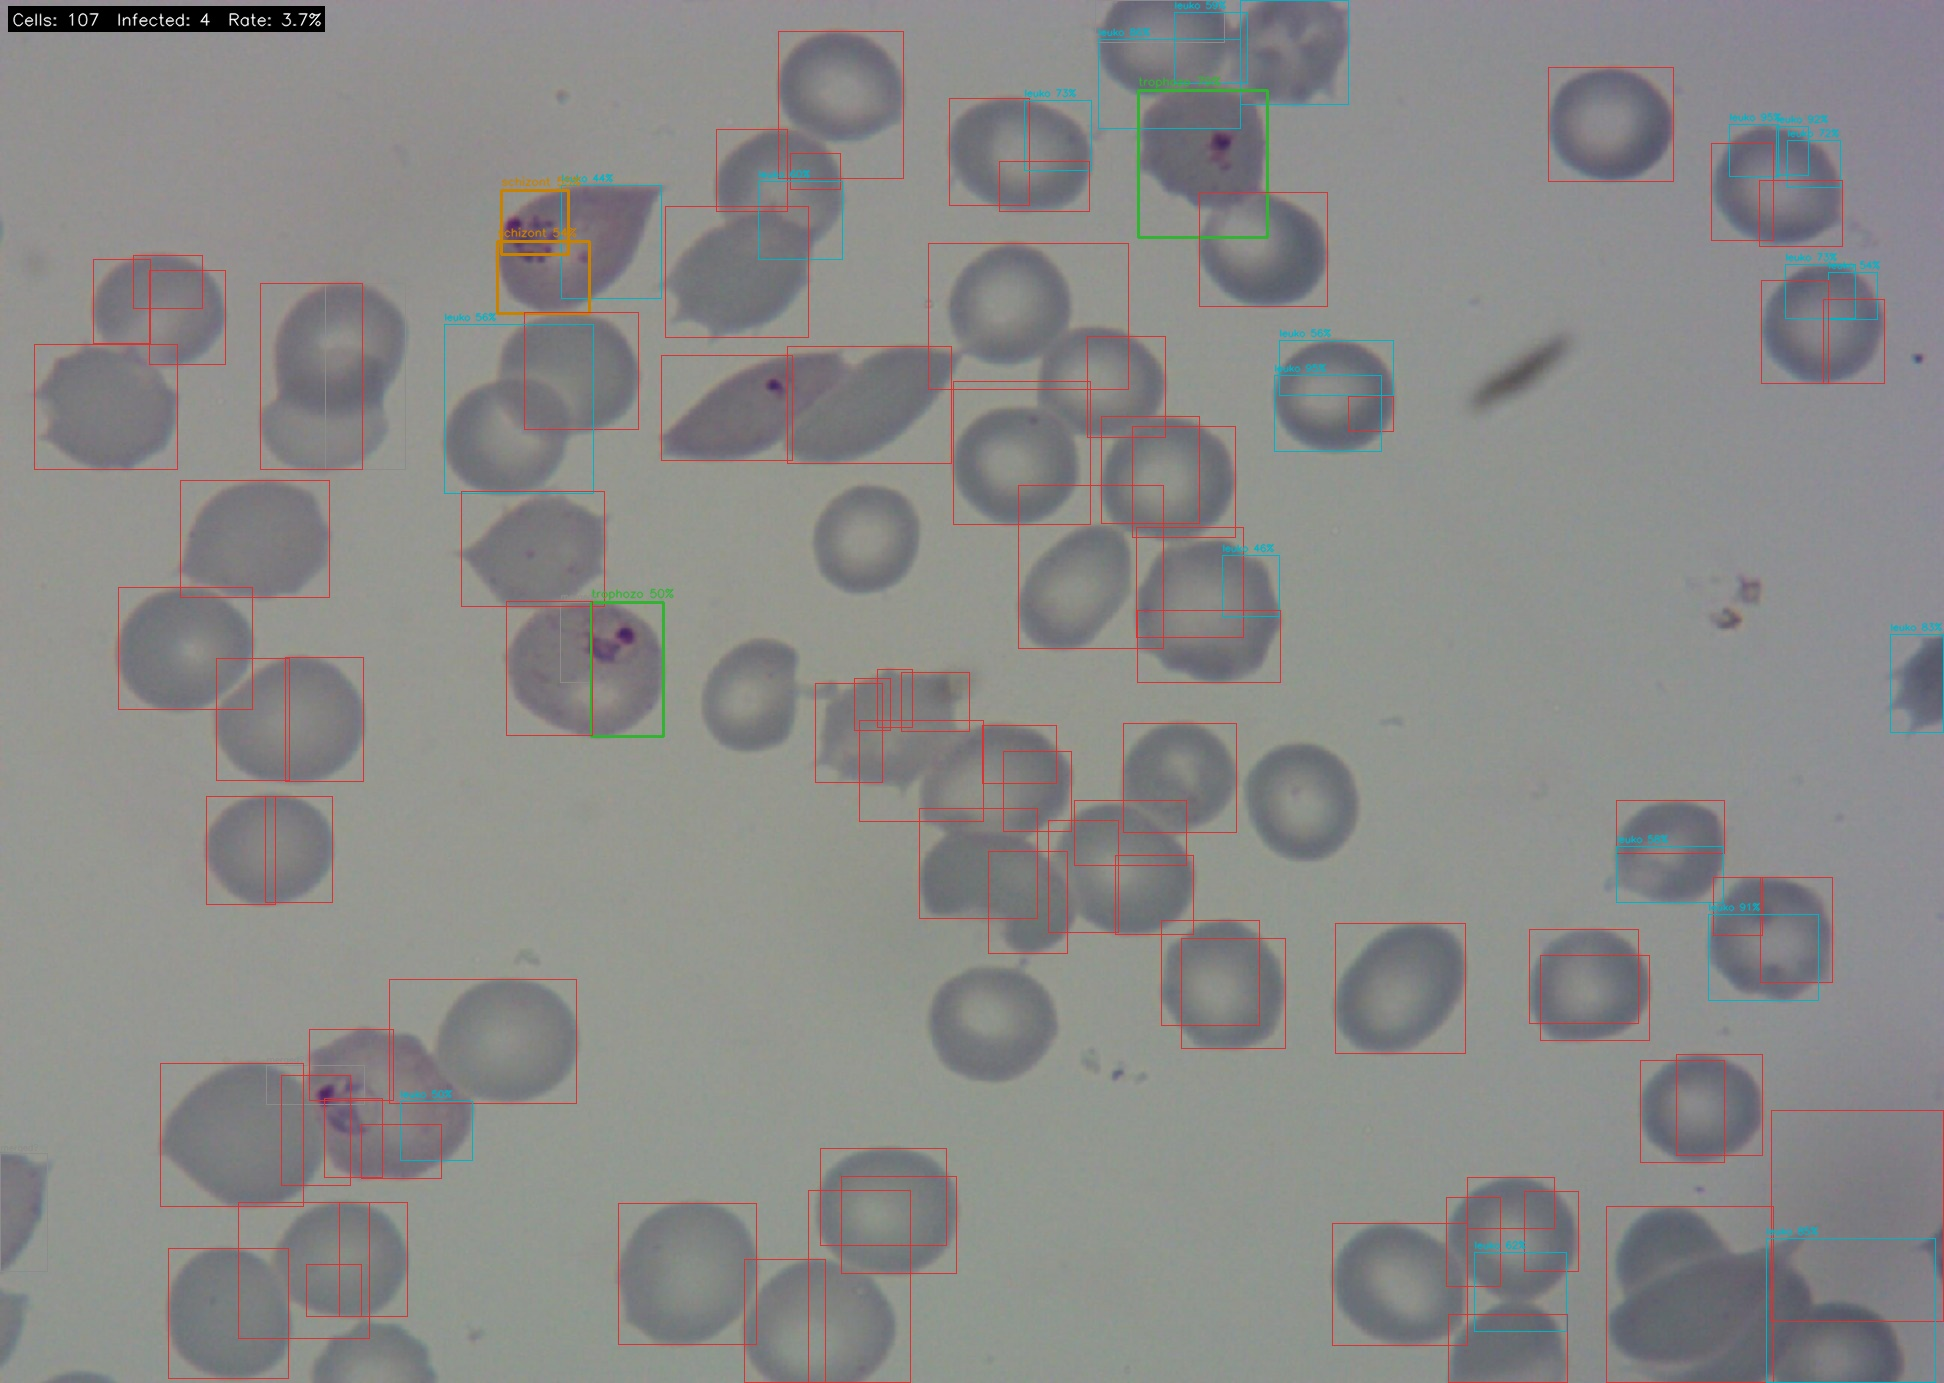
\includegraphics[width=\linewidth]{fig_appendix_iter2.jpg}
  \caption{Iteration~2 output: size filter applied. Noise eliminated;
    oversized merged-cluster regions remain unlabelled.}
  \label{fig:appendix_iter2}
\end{figure}

\subsection*{Iteration 3 (Final) --- Stable Pipeline}

The final iteration introduces explicit flagging of oversized merged regions
and a confidence threshold of 0.40 on parasite predictions. This is the
pipeline described in Section~\ref{ssec:stage1} and evaluated in
Section~\ref{ssec:stage1_results}.

\end{document}
